\documentclass{headers/polimi_3i}

%------------------------------------------------------------------------------
%	REQUIRED PACKAGES AND  CONFIGURATIONS
%------------------------------------------------------------------------------

% CONFIGURATIONS
\usepackage{parskip} % For paragraph layout
\usepackage{setspace} % For using single or double spacing
\usepackage{emptypage} % To insert empty pages
\usepackage{multicol} % To write in multiple columns (executive summary)
\setlength\columnsep{15pt} % Column separation in executive summary
\setlength\parindent{0pt} % Indentation
\raggedbottom  

% PACKAGES FOR TITLES
\usepackage{titlesec}
% \titlespacing{\section}{left spacing}{before spacing}{after spacing}
\titlespacing{\section}{0pt}{3.3ex}{2ex}
\titlespacing{\subsection}{0pt}{3.3ex}{1.65ex}
\titlespacing{\subsubsection}{0pt}{3.3ex}{1ex}
\usepackage{color}

% PACKAGES FOR LANGUAGE AND FONT
\usepackage[english]{babel} % The document is in English  
\usepackage[utf8]{inputenc} % UTF8 encoding
\usepackage[T1]{fontenc} % Font encoding
\usepackage[11pt]{moresize} % Big fonts

% PACKAGES FOR IMAGES
\usepackage{graphicx}
\usepackage{transparent} % Enables transparent images
\usepackage{eso-pic} % For the background picture on the title page
%\usepackage{subfig} % Numbered and caption subfigures using \subfloat.
\usepackage{tikz} % A package for high-quality hand-made figures.
\usetikzlibrary{}
\graphicspath{{./images/}} % Directory of the images
\usepackage{caption} % Coloured captions
\usepackage{subcaption} % Subfigures
\usepackage{xcolor} % Coloured captions
\usepackage{amsthm,thmtools,xcolor} % Coloured "Theorem"
\usepackage{float}

% STANDARD MATH PACKAGES
\usepackage{amsmath}
\usepackage{amsthm}
\usepackage{amssymb}
\usepackage{amsfonts}
\usepackage{bm}
\usepackage[overload]{empheq} % For braced-style systems of equations.
\usepackage{fix-cm} % To override original LaTeX restrictions on sizes

% PACKAGES FOR TABLES
\usepackage{tabularx}
\usepackage{longtable} % Tables that can span several pages
\usepackage{colortbl}

% PACKAGES FOR ALGORITHMS (PSEUDO-CODE)
\usepackage{algorithm}
\usepackage{algpseudocode}

% PACKAGES FOR REFERENCES & BIBLIOGRAPHY
\usepackage[colorlinks=true,linkcolor=black,anchorcolor=black,citecolor=black,filecolor=black,menucolor=black,runcolor=black,urlcolor=black]{hyperref} % Adds clickable links at references
\usepackage{cleveref}
%\usepackage[square, numbers, sort&compress]{natbib} % Square brackets, citing references with numbers, citations sorted by appearance in the text and compressed
%\bibliographystyle{abbrvnat} % You may use a different style adapted to your field

% OTHER PACKAGES
\usepackage{pdfpages} % To include a pdf file
\usepackage{afterpage}
\usepackage{lipsum} % DUMMY PACKAGE
\usepackage{fancyhdr} % For the headers

\fancyhf{}

% Input of configuration file. Do not change config.tex file unless you really know what you are doing. 
% Define blue color typical of polimi
\definecolor{bluepoli}{cmyk}{0.4,0.1,0,0.4}

% Custom theorem environments
\declaretheoremstyle[
  headfont=\color{bluepoli}\normalfont\bfseries,
  bodyfont=\color{black}\normalfont\itshape,
]{colored}

% Set-up caption colors
\captionsetup[figure]{labelfont={color=bluepoli}} % Set colour of the captions
\captionsetup[table]{labelfont={color=bluepoli}} % Set colour of the captions
\captionsetup[algorithm]{labelfont={color=bluepoli}} % Set colour of the captions

\theoremstyle{colored}
\newtheorem{theorem}{Theorem}[chapter]
\newtheorem{proposition}{Proposition}[chapter]

% Enhances the features of the standard "table" and "tabular" environments.
\newcommand\T{\rule{0pt}{2.6ex}}
\newcommand\B{\rule[-1.2ex]{0pt}{0pt}}

% Pseudo-code algorithm descriptions.
\newcounter{algsubstate}
\renewcommand{\thealgsubstate}{\alph{algsubstate}}
\newenvironment{algsubstates}
  {\setcounter{algsubstate}{0}%
   \renewcommand{\STATE}{%
     \stepcounter{algsubstate}%
     \Statex {\small\thealgsubstate:}\space}}
  {}

% New font size
\newcommand\numfontsize{\@setfontsize\Huge{200}{60}}

% Title format: chapter
\titleformat{\chapter}[hang]{
\fontsize{50}{20}\selectfont\bfseries\filright}{\textcolor{bluepoli} \thechapter\hsp\hspace{2mm}\textcolor{bluepoli}{|   }\hsp}{0pt}{\huge\bfseries \textcolor{bluepoli}
}

% Title format: section
\titleformat{\section}
{\color{bluepoli}\normalfont\Large\bfseries}
{\color{bluepoli}\thesection.}{1em}{}

% Title format: subsection
\titleformat{\subsection}
{\color{bluepoli}\normalfont\large\bfseries}
{\color{bluepoli}\thesubsection.}{1em}{}

% Title format: subsubsection
\titleformat{\subsubsection}
{\color{bluepoli}\normalfont\large\bfseries}
{\color{bluepoli}\thesubsubsection.}{1em}{}

% Shortening for setting no horizontal-spacing
\newcommand{\hsp}{\hspace{0pt}}

\makeatletter
% Renewcommand: cleardoublepage including the background pic
\renewcommand*\cleardoublepage{%
  \clearpage\if@twoside\ifodd\c@page\else
  \null
  \AddToShipoutPicture*{\BackgroundPic}
  \thispagestyle{empty}%
  \newpage
  \if@twocolumn\hbox{}\newpage\fi\fi\fi}
\makeatother

%For correctly numbering algorithms
\numberwithin{algorithm}{chapter}

%----------------------------------------------------------------------------
%	NEW COMMANDS DEFINED
%----------------------------------------------------------------------------

%----------------------------------------------------------------------------
%	ADD YOUR PACKAGES (be careful of package interaction)
%----------------------------------------------------------------------------

\usepackage{enumitem}

\usepackage[style=numeric, sorting=nyt]{biblatex}

\addbibresource{chapters/biblio.bib}

%----------------------------------------------------------------------------
%	ADD YOUR DEFINITIONS AND COMMANDS (be careful of existing commands)
%----------------------------------------------------------------------------

%todo box highlight
\newcommand{\TODO}[1]{\noindent\colorbox{orange}{
	\parbox{\dimexpr\linewidth-2\fboxsep}
	{\textcolor{black}{\textbf{TODO:} #1}}}\par}

% Define a custom command for the list inside a table
% inserts padding on top and bottom, and no left indentation
\newcommand{\customtablelist}[1]{%
	\noindent
	\begin{minipage}[c]{6cm}
		\raggedright
		\begin{itemize}[left=0pt, after=\strut, before=\vskip 8pt]
			#1
		\end{itemize}
	\end{minipage}
}

\hyphenation{Interpret-ability}

%----------------------------------------------------------------------------
%	BEGIN OF YOUR DOCUMENT
%----------------------------------------------------------------------------

\begin{document}

\fancypagestyle{plain}{%
\fancyhf{} % Clear all header and footer fields
\fancyhead[RO,RE]{\thepage} %RO=right odd, RE=right even
\renewcommand{\headrulewidth}{0pt}
\renewcommand{\footrulewidth}{0pt}}




\startpreamble
\setcounter{page}{1} % Set page counter to 1
\addtocontents{toc}{\vspace{2em}} % Add a gap in the Contents, for aesthetics
\mainmatter % Begin numeric (1,2,3...) page numbering

\chapter{Experimental Setups and Demonstrations}

This chapter will describe the experiments conducted to demonstrate the capabilities of the mobile manipulation
robotic system. The experiments consist of three demonstrations named "ArUco Follower", "Button Presser", and "Object Picking".
These demos are meant to showcase the capabilities of the robot in various tasks such as following
a marker, pressing buttons, and picking objects. The first demo is a preview of the robotic arm's
autonomous control software. The second demo showcases the capabilities of the entire system in performing
high-level tasks in industrial environments, such as pressing buttons on an industrial control panel.
The third demo is meant to showcase the mobile manipulation capabilities in an agricultural environment, such as picking
fruits.

The experiments are conducted in a controlled realistic environment to test the robustness
and reliability of the system. The demos have been tested inside the Artificial Intelligence and Robotics Laboratory
at Politecnico di Milano. The laboratory has enough space to allow testing the efficiency of the autonomous 
navigation software while testing also the obstacle avoidance algorithm in a cluttered and changing environment.

The objectives of these demonstrations are to evaluate the robot's performance within the
various software components and how well they integrate with the hardware components. The experiments will also
highlight the challenges faced during the development and testing of the robotic system and how they were overcome.
The demos are meant to be a proof of concept of the robotic system's capabilities in simulated scenarios that are as close as
possible to more realistic environments. They are also meant to show the potential of mobile manipulation 
robots in performing various complex tasks that are currently performed by humans. The objective is not to
replace humans but to assist them in performing tasks that are dangerous, repetitive, or require high precision.

\section{ArUco Follower Demo}

The ArUco Follower demo is a demonstration of the robotic arm's autonomous control software. The demo
consists of the robotic arm following an ArUco marker with the end effector. The demo showcases the
motion planning and execution libraries with MoveIt2 and the integration of the ArUco marker detection 
and pose estimation algorithms with the robotic arm's control software.
The demo tests the autonomous control software of the robotic arm in tracking and following a moving target.
Figure \ref{fig:arucofollower} shows the demo in execution, with \textit{MountV1} as end effector (but without
the cylinder presser). The cardboard shown to the camera displays an ArUco marker, tracked by the robotic arm.

In this demo, the end effector, equipped with the camera, will move in a position and orientation that points
toward the center of the
ArUco marker. The algorithm for \textbf{tracking the marker} computes the end effector's target position such that
the arm can always reach it, and the orientation of the end effector is always pointing towards the marker.
The position of the end effector will be exactly the marker's position if the marker is sufficiently close to the arm,
otherwise, the end effector will be positioned to point the camera toward the marker.
If the marker is not visible, the end effector will remain in the last known position until the marker is
visible again. If the marker moves to a different position in the camera frame and stays visible,
the algorithm will compute the new target pose and the end effector will move to it.
The computation of the end effector's target pose is based on geometrical calculations from the marker's position
in the camera frame. The marker's pose is transformed in the robot arm's base frame, and the target pose is
computed based on the robotic arm's workspace. The target pose is then sent to the motion planning and execution
libraries to compute and execute the trajectory to reach the target pose.

A demonstration incorporating the MoveIt2 Servo node for real-time end-effector control via ArUco marker pose
targeting was implemented and tested. However, due to the ongoing development of MoveIt2 Servo at the time of
writing and its associated stability limitations, the resulting trajectories exhibited undesirable jerkiness 
and did not consistently achieve the target pose within a short timeframe. 
Additionally, the requirement for precise PID tuning of the closed-loop joint trajectory controller presented further
challenges in achieving optimal real-time performance. Given these constraints, the decision was made to utilize 
the standard MoveIt2 planning and execution libraries for the final demonstration,
ensuring greater reliability and smoother operation.

% Add a Figure of the ArUco Follower demo setup during testing
\begin{figure}[t]
    \centering
    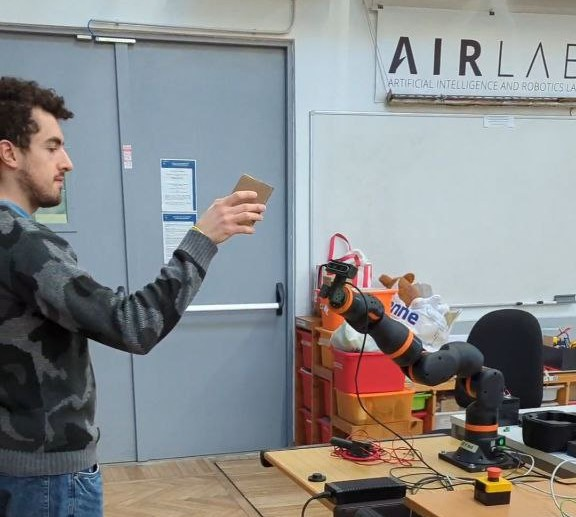
\includegraphics[width=0.7\textwidth]{c5_19.jpg}
    \caption{ArUco Follower demo during execution. The cardboard shows an ArUco marker.}
    \label{fig:arucofollower}
\end{figure}

\section{Button Presser Demo}

The "Button Presser" demo is a complex demonstration that showcases the potential of mobile manipulation robots
in performing high-level tasks in industrial environments. The demo consists of the robotic arm pressing buttons
on an industrial control panel, in an autonomous way. The objective is to show the capabilities of the robot in performing
tasks that are currently performed by humans. The demo is meant to be a proof of concept of the robotic system's
integration of multiple software components and the orchestration of the robotic arm and mobile base to
interact with the environment without human intervention.
The demo was developed in the context of a larger project in collaboration with a company. The aim of the project is
to use mobile manipulation robots in industrial plants, for monitoring sensors and various equipment,
and intervening in case of emergency, while avoiding human intervention in dangerous environments. 

The purpose is to demonstrate the feasibility of the mobile manipulation robot in interacting with the control panel
autonomously and effectively. It was also important to demonstrate the system's reliability and robustness 
in performing such a complex task, in terms of accuracy in pressing buttons and the time taken to press all the buttons.

\subsection{Buttons Setup Box and End Effector Setups}

For this demo, the \textit{MountV1} was employed, mounted on the robotic arm's end effector. The \textit{MountV1} is a 
custom-designed 3D-printed mount attached to the cobot's flange, which allows the installation of the stereo camera and 
the cylinder presser. The cylinder presser is a cylinder-shaped tool used for pressing buttons.
In \textit{MountV1} the camera is placed in front of the flange, and this resulted in a reduced field of view of the camera.
Despite this camera position, the camera was able to detect the ArUco markers on the control panel
and the buttons to be pressed. Since the \textit{MountV1} proved to be quite effective in the demo, 
the only change made to this version was to shorten the cylinder presser to prevent
the mobility of the end effector from being reduced due to the length of the tool.

Further in the development of the demo, the end effector configuration was switched to \textit{MountV2}, 
which is the next version of \textit{MountV1}. The biggest improvement of \textit{MountV2} is the camera's position, 
which is placed on the wrist of the cobot, allowing a greater field of view of the camera. 
This proved more effective in finding the ArUco markers on the control panel from a closer distance. 

Using \textit{MountV1}, the end effector was slipping during the execution of the linear trajectories, due to the
roundness of the button caps. This is due to the low friction between the digital button and the round button cap,
having both surfaces made of plastic and a small contact area. The slipping of the end effector caused the
robotic arm to fail to press the buttons effectively. To overcome this problem, the end effector was replaced
with \textit{MountV2}, which has a vacuum suction cap on its tip, instead of having a cylinder presser.
The end effector presents a vacuum suction capo used to press the buttons effectively.
This solution is more effective in pressing the buttons, thanks to the greater friction between the plastic
button cap and the silicon suction cup. The vacuum suction cap presses the buttons reliably, with less slipping,
thanks also to the greater contact area between the cap and the button.

%\TODO{add picture comparison between MountV1 and MountV2 end effectors}

The Realsense camera was used only for ArUco markers detection and pose estimation. So the software
component related to the perception of the control panel didn't make use of the infrared cameras for 
depth estimation. The position of the markers is in fact computed using the RGB image as input and
the equations for 3D camera projection on a 2D matrix for the pose estimation.

The control panel is a custom-designed box with three buttons of different sizes and seven ArUco markers
(having dictionary 4x4) placed around the buttons. Figure \ref{fig:buttonsbox} shows the control panel.
The control panel is small and portable and can be placed in any position and orientation to test the robustness
of the system. The control panel has also three different lights, one for each button,
that indicate whenever a button is pressed. 

The reason for having multiple ArUco markers instead of just one or three for the three buttons,
is to have a more robust and reliable detection of the buttons' positions. Having multiple markers
allows the system to detect the buttons' orientation in a more precise way that is also robust to noise.
The markers are placed around the buttons in a way that the plane estimation algorithm can compute
the plane of the markers effectively, relying on a greater number of points to estimate the plane.

\begin{figure}[t]
    \centering
    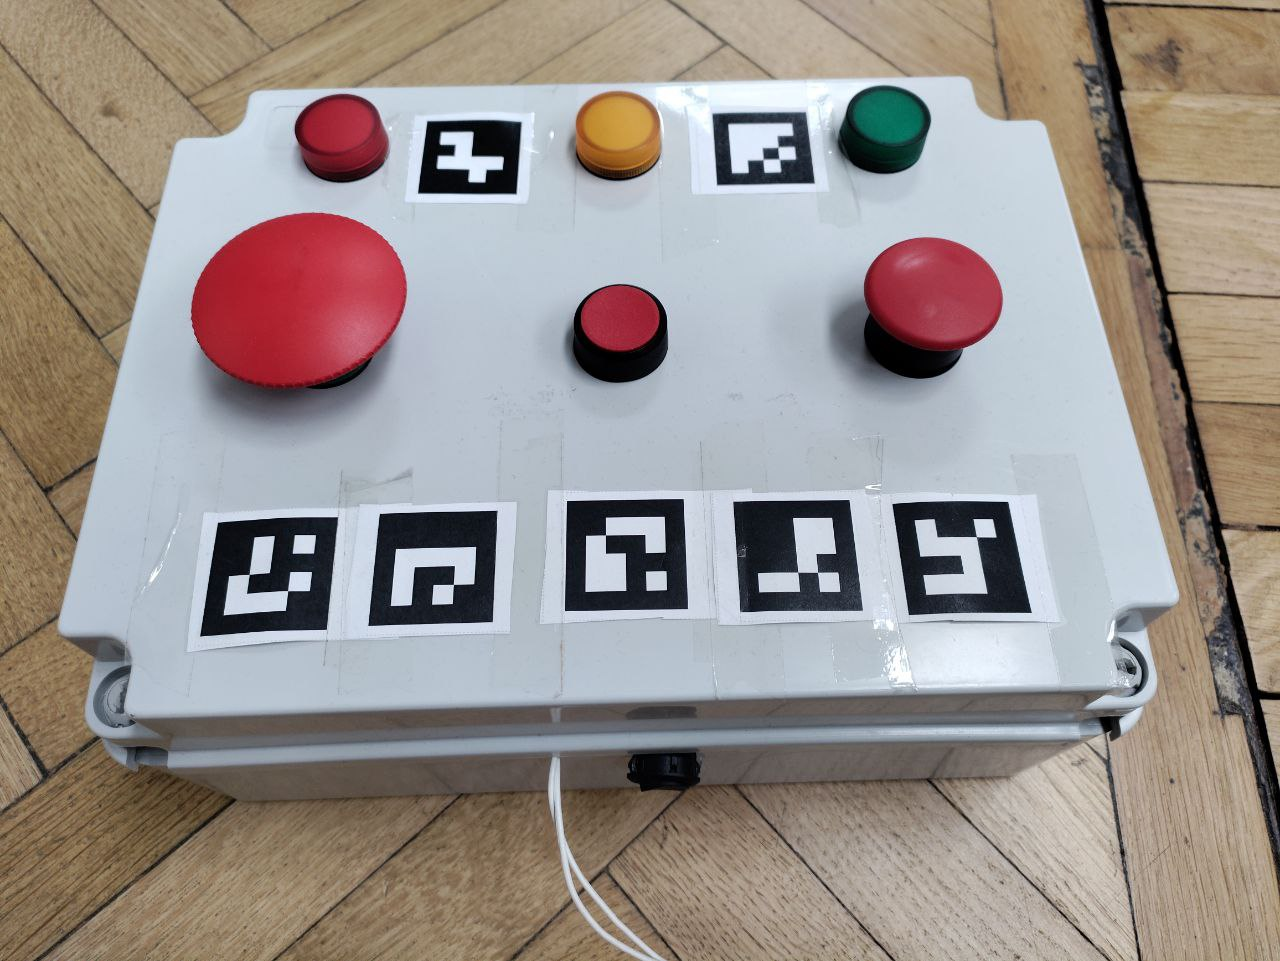
\includegraphics[width=0.7\textwidth]{c5_05.jpg}
    \caption{Control panel with 3 buttons and ArUco markers.}
    \label{fig:buttonsbox}
\end{figure}

\subsection{End Effector Positioning and Linear Trajectories}

The implementation of the algorithms for pressing buttons and planning the trajectories is handled inside
ROS2 nodes. One ROS2 node subscribes to the ArUco markers detection topic containing the estimated markers' poses 
and their IDs. Given the markers' poses, and the relative positioning of the markers with respect to the buttons,
the node computes the position of the buttons in the robot's base frame. The node also computes the orientation
of the end effector, such that the vector from the arm's flange and the end effector tip
faces the plane of the markers orthogonally, and this is needed to compute the orientation required to press the buttons.

The \textbf{algorithm} for computing the sequence of target poses that the end effector must reach uses the 
\textbf{estimated position and orientation of the buttons}. For each button, the algorithm computes the pose 
immediately above the button, meaning that the end effector faces the button orthogonally from a fixed distance.
Then the algorithm generates the linear path that the end effector must follow to reach the pose where 
the button is pressed. The linear path is then reversed to get the path required to lift the end effector 
from the button in order to release it and return to the starting point above the button. This sequence
of target poses computation is repeated for each button on the control panel. The ROS2 node uses these target 
poses and linear paths to plan and generate the trajectories for the arm to reach the target poses and 
follow the linear paths. Once the trajectory plans are generated, they are executed.

The linear motion trajectory generation is the most challenging part of the trajectory planner,
because the algorithm that computes the trajectories must take into account several constraints,
such as the static collisions with external bodies and the robotic arm's self-collision mapping.
There are two main methods to generate a linear trajectory for the end effector in cartesian space:

\begin{itemize}
    \item \textbf{Cartesian Linear Motion Planning generation via a sequence of waypoints}:
    this method generates a sequence of pose waypoints (sequence of positions and orientation) that the
    end effector must follow to reach the target pose. The trajectory is generated by interpolating
    the sequence of waypoints in space and time. The trajectory planner generates a trajectory that
    follows the waypoints with maximum deviation defined as the \textit{end effector jump}, which is
    the maximum total deviation in joint space that each joint can have from the average joints' positions.
    This parameter controls how much the joints can move from their average configuration during the 
    execution of the linear trajectory. Setting the end effector jump to zero means that the joints
    will not move from their average configuration, and the end effector will follow the waypoints
    exactly.
    \item \textbf{Constrained Cartesian Motion Planning}: this method creates a motion plan request with the
    addition of position and orientation constraints on the end effector that must be respected while moving
    toward the final pose. The constraints are defined as a position box constraint, meaning that the end 
    effector must stay within a box (rectangular cuboid) in the cartesian space, and an orientation constraint,
    defined as a quaternion representing the orientation and the maximum angle of deviation from the
    orientation axis defined by the quaternion.
\end{itemize}

Both methods were tested and implemented successfully to be used with the Igus Rebel cobot.
The constrained cartesian motion planning method proved to be unreliable due to the high probability
of not being able to generate a valid trajectory. Adding only one constraint to the motion plan made
the trajectory planner able to find a solution most of the time. But adding two constraints, one for 
the position and one for the orientation, resulted in failed trajectory generation almost every time.
This limitation is caused by the physical characteristics of the robotic arm. To successfully generate
a constrained cartesian motion plan, the robotic arm must have 7 DoF, while the Igus Rebel cobot has only 6 DoF.
This makes the constrained method not suitable for this robotic arm.
The reason behind this is that constraining a motion plan 
with two constraints for a 6-DoF robotic arm results in an overdetermined system of equations, and the
trajectory planner is not able to find a feasible solution, because the constraints add more equations 
than the number of DoF of the robotic arm, resulting in a system of equations with no feasible solution.

Due to this limitation, only the cartesian linear motion planning method was used to generate linear trajectories
following a sequence of waypoints. The end effector's jump was set to zero to make the end effector follow
the waypoints exactly, to avoid random jumps in the cobot's configuration. The linear trajectories were
generated successfully and executed correctly most of the time. Sometimes the trajectory planner failed
to find a solution, even when attempting to create a trajectory plan multiple times. This was due to the
complexity of the environment that the planner must take into account. After many attempts with 
different motion planners, such as OMPL, STOMP, and the Pilz industrial motion planner, the one that
proved to be the most reliable and robust for generating linear trajectories was the Pilz industrial motion planner.

The \textbf{reliability of the trajectory planner} in generating linear trajectories for the end effector
was a crucial aspect of the demo and posed a challenge during the development and testing of the demo.
The planner failed to find a feasible solution frequently. In order to increase the probability of finding
a feasible solution, an increase in the tolerances of the planner, such as the maximum deviation
of the end effector from the waypoints, and an increase in the number of attempts to generate a trajectory plan
made the planner more reliable.

\subsection{Mobile Button Presser Demo}

The "mobile button presser" demo is a complex demonstration to showcase the mobile manipulation robot's
capabilities in pressing buttons on an industrial control panel autonomously. The demo consists of the mobile
manipulation robot navigating to the control panel's location, detecting the control panel, and pressing the buttons
in a predefined sequence.

The \textbf{complete demo}, illustrated in the flowchart in Figure \ref{mbp_flowchart}, consists of the following steps:
\begin{enumerate}
    \item The mobile manipulation robot starts from a random location and does not know 
    where the control panel is located.
    \item The robotic arm performs an inspection routine using the camera mounted on the end effector
    to search for a specific ArUco marker, which signals where the control panel is located.
    \item Once the specified marker is detected, and its distance is computed, the algorithm computes the
    position of the control panel in the map frame of reference.
    \item The robotic arm parks itself to not obscure the field of view of the LiDAR, which is essential for 
    localization and autonomous navigation.
    \item The mobile base navigates to the control panel's location autonomously, while avoiding obstacles in the
    environment.
    \item The mobile robot parks in front of the control panel at a fixed distance, facing the opposite side of the control panel,
    so that the robotic arm can move freely without colliding with the mobile base and reach the buttons.
    Figure \ref{fig:buttonpresser1} shows this stage of execution of the demo.
    \item The robotic arm uses the onboard camera mounted on the end effector to inspect the close environment
    to search for the ArUco markers on the control panel, indicating the locations of the buttons to be pressed.
    \item Once the camera detects the ArUco markers, the algorithm computes the position and orientation
    of the buttons placed on the panel in the robot's base frame.
    \item For each button, it finds the end effector target poses in the cartesian space required to press the buttons.
    It also creates the linear paths for the end effector necessary to press and release the buttons.
    \item The robotic arm executes the computed trajectories, and the end effector presses the buttons in the predefined sequence.
    Figure \ref{fig:buttonpresser2} shows the end effector pressing one of the buttons, at this stage of execution of the demo.
    \item The control panel lights up the corresponding light for each pressed button.
\end{enumerate}

\begin{figure}[t]
    \centering
    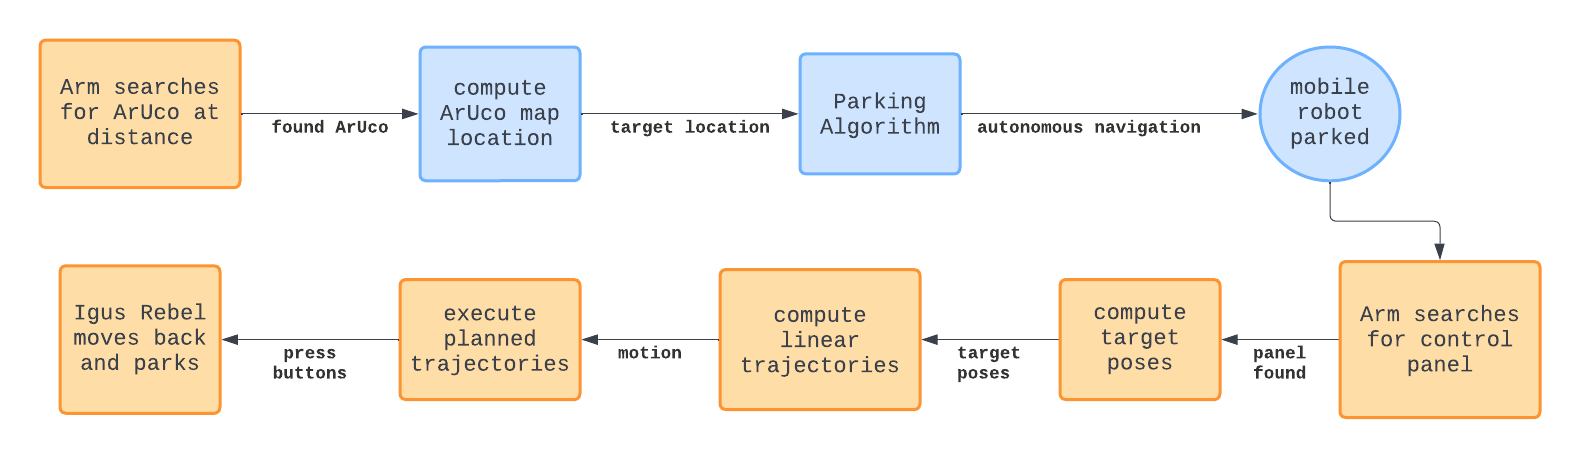
\includegraphics[width=1.0\textwidth]{demo1.png}
    \caption{Flowchart of the Mobile Button Presser demo execution}
    \label{mbp_flowchart}
\end{figure}

\subsection{Mobile Button Presser Demo Implementation and Architecture}
\label{sec:demo1}

This demonstration is handled by one ROS2 node (action client) that orchestrates the actions of the mobile base
and the robotic arm. The client node sends the goal to three different action servers:

\begin{itemize}
    \item \textbf{Parking Action Server}: this server is responsible for computing the parking algorithm, given the
    position of the control panel in the map frame. After the parking pose is computed, the server sends a navigation
    goal to the nav2 stack to navigate autonomously to the parking pose. The action returns the result containing
    information about how close the robot is to the parking pose when the autonomous navigation is completed.
    \item \textbf{Button Finder Action Server}: this server is responsible for searching for a specific ArUco marker
    in the room. The server executes a "searching movement", which is a sequence of predefined poses that the robotic arm
    must follow to search for the marker. The server also executes all trajectories until the marker is detected.
    The server returns once the marker is detected, and the distance from the cobot to the marker is computed.
    \item \textbf{Button Presser Action Server}: this server is responsible for pressing the buttons on the control panel.
    It first computes the "searching movement" to search for the ArUco markers on the control panel.
    Once the markers are detected and the control panel is located, the server computes the target poses and linear paths
    for pressing the buttons. The server then executes the trajectories to press the buttons in the predefined sequence.
    The server keeps track of how many trajectories have been planned and successfully executed, with respect to
    the total number of trajectories to be executed. The server returns the success rate of the executed trajectories.
    The server terminates its execution once all the buttons have been pressed.
\end{itemize}

% Add pictures of the demo execution
\begin{figure}[t]
    \centering
    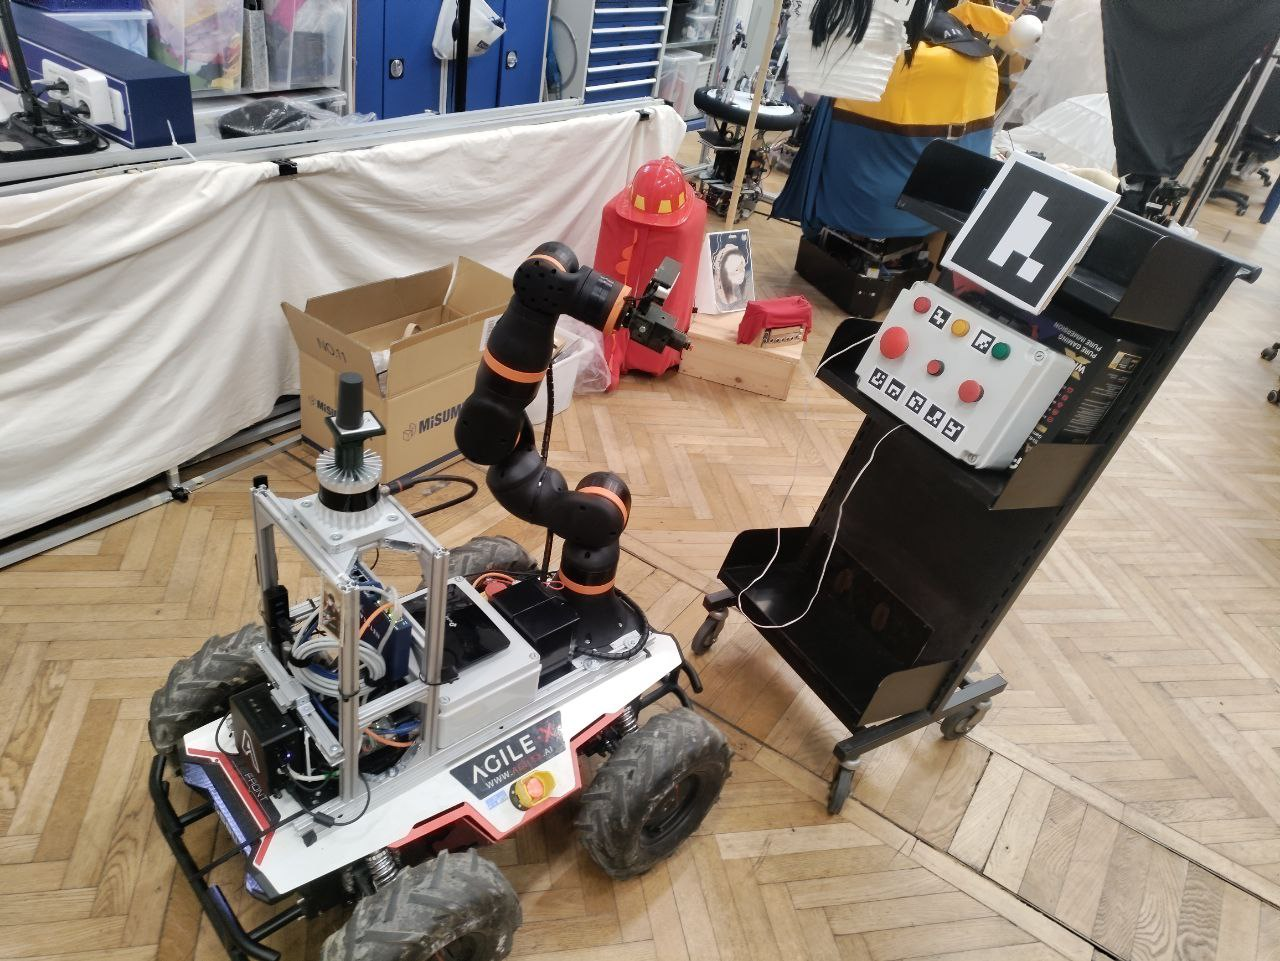
\includegraphics[width=1.0\textwidth]{c5_10.jpg}
    \caption{Mobile Button Presser Demo in execution}
    \label{fig:buttonpresser1}
\end{figure}

\begin{figure}[t]
    \centering
    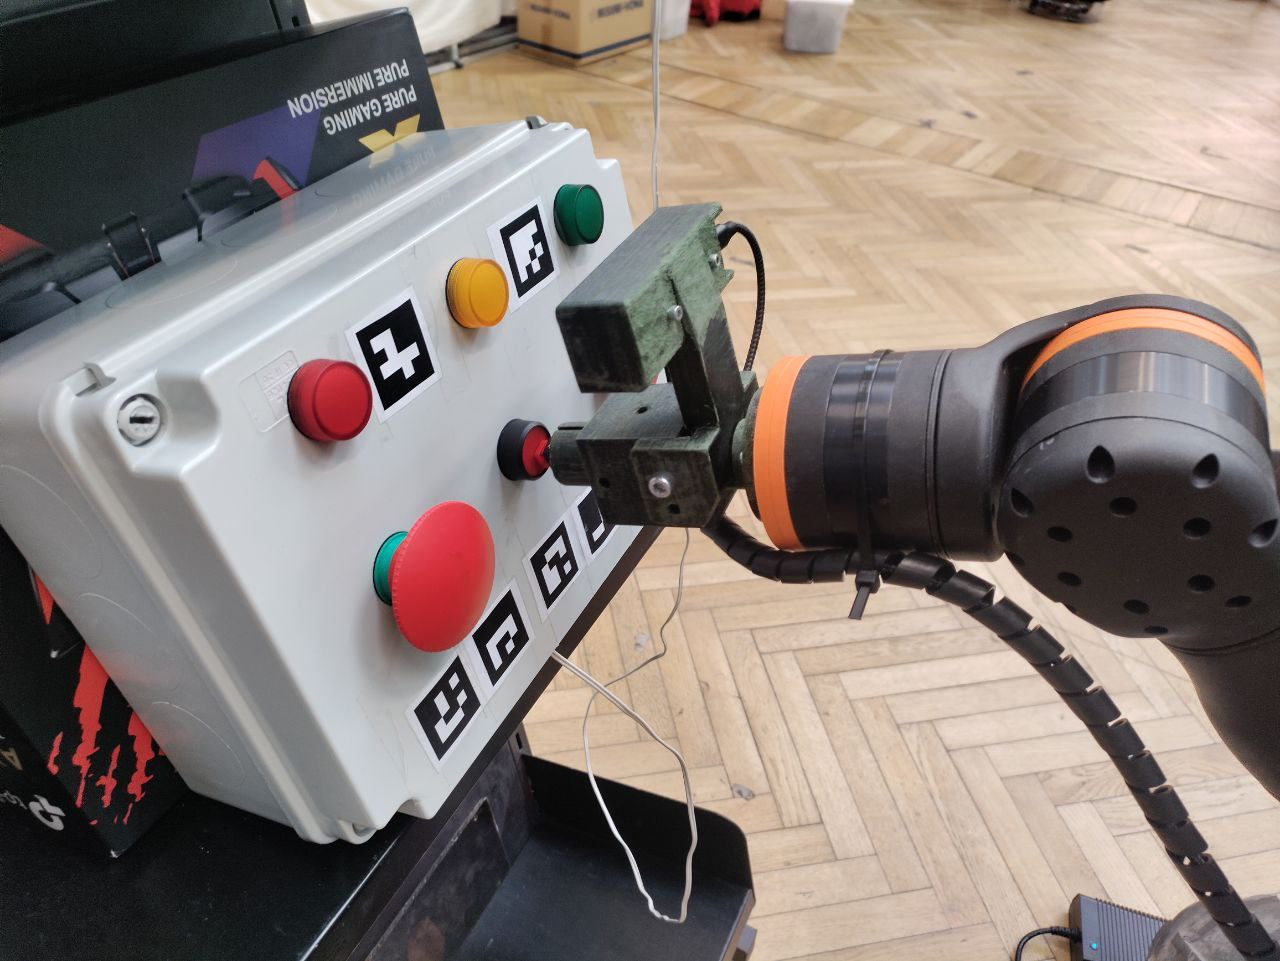
\includegraphics[width=1.0\textwidth]{c5_12.jpg}
    \caption{Cobot pressing buttons on the control panel using the \textit{MountV1} end effector}
    \label{fig:buttonpresser2}
\end{figure}

The architecture of the whole system is composed of multiple software components that interact with each other
using ROS2 Actions and Topics. The architecture, shown in Figure \ref{fig:arch1}, is designed to be modular
and scalable, to allow the integration of new components and functionalities in the future.
The architecture is composed of the following macro components:

\begin{itemize}
    \item \textbf{Multi-ArUco Plane Detection and Marker Pose Estimation}: this component is responsible for detecting
    the ArUco markers in the camera's field of view and estimating the markers' poses. The component relies on 
    the Multi-ArUco Plane Detection algorithm to detect the markers and correct their estimated poses using the
    plane estimation algorithm. This algorithm is explained in section \ref{sec:multiaruco}.
    The component publishes the markers' corrected poses on a ROS2 topic.
    \item \textbf{MoveIt2 Servers}: this component includes the MoveIt2 Planning and Execution functionalities
    and the two action servers for finding the parking pose and pressing the buttons. The MoveIt2 servers
    are responsible also for computing and executing the linear trajectories generated by the trajectory planner,
    required to press the buttons. The demo execution pipeline is handled within threads executed 
    on-demand by the MoveIt2 servers, given the goal sent by the client node.
    \item \textbf{Nav2 Servers}: this component is responsible for the autonomous navigation of the mobile base
    using Nav2. It includes also the action server for computing the parking algorithm and the action client
    exploiting Nav2 Commander APIs to send navigation goals to the mobile base. The structure of the parking algorithm
    is explained in section \ref{sec:parking}, while the autonomous navigation integration with ROS2 is explained
    in section \ref{sec:nav2}.
    \item \textbf{Client Node}: this component is responsible for orchestrating the actions of the mobile base
    and the robotic arm. The client node is a ROS2 node that integrates the action clients for the parking, button finder,
    and button presser action servers. The orchestration of the actions is handled by different threads that
    are executed on-demand by the client node, given the goal sent by the user. Multiple threads are present
    since each one is responsible for handling different tests and demo versions.
\end{itemize}

% Add a Picture of the diagram
\begin{figure}[t]
    \centering
    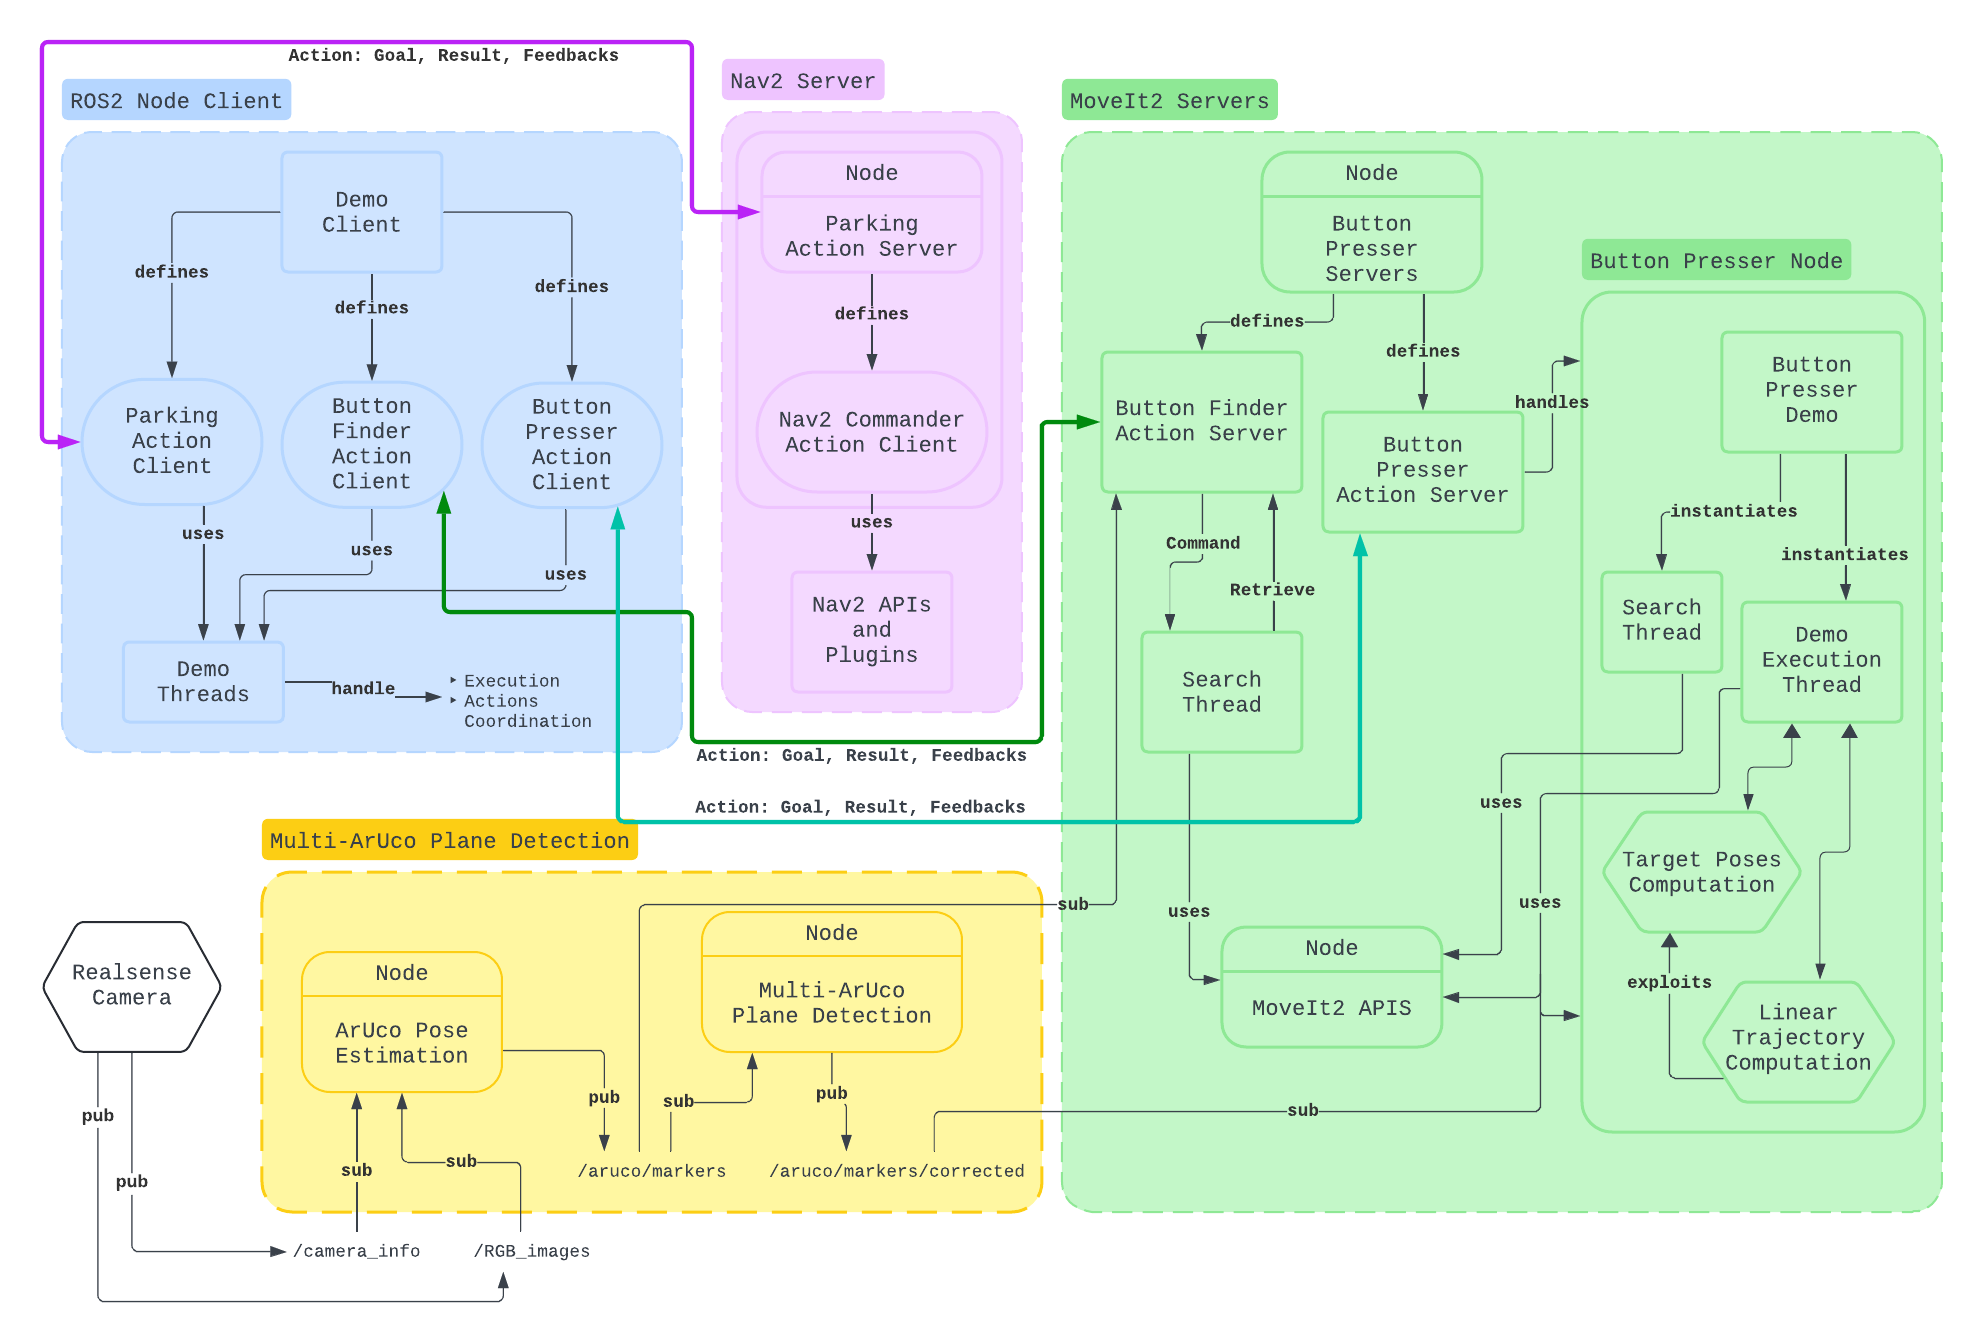
\includegraphics[width=1.0\textwidth]{Mobile Button Presser Demo_updated.png}
    \caption{Architecture diagram of the Mobile Button Presser demo}
    \label{fig:arch1}
\end{figure}


\section{Object Picking Demo}

The "Object Picking" demo is a more complex demonstration that showcases the mobile manipulation robot's capabilities
in picking objects from the environment autonomously. The demo consists of the robotic arm picking colored balls
or apples from an artificial plant, autonomously. The objective is to demonstrate the robotic system's integration of
multiple software components and the orchestration of the robotic arm and mobile base to interact and grasp objects of
different shapes and sizes, using a soft robotic hand gripper.
The soft gripper enables the robotic arm to grasp fragile objects without damaging them, and it is also able to
grasp objects of different shapes and sizes, thanks to the flexibility and adaptability of the silicone fingers.
For this demo, the \textit{MountV2} is used, since it is the only one that supports the soft gripper.

The colored balls used in the demo are small plastic balls of different colors. The balls are used as a
test ground for the grasping capabilities of the soft gripper since they are small enough to be easy to grasp
and the plastic material enables high friction between the fingers and the ball. Instead, the artificial apples
are a little more challenging to grasp, because of their irregular shape.
The artificial apples are used to simulate a realistic and more complex scenario, where the objects to be picked are
closer to objects appearing in real-world environments, such as fruits on trees.

The \textbf{objective of the demo} is to apply the mobile manipulation robot in an agricultural environment, which is
often more challenging and irregular than in industrial environments. The demo is meant to be a proof of concept
of the autonomous control of a robot to pick and place objects in a realistic environment, such as a plantation.

For this demo, three different versions were developed, each with different levels of complexity and challenges.
The first version is used as a test for the algorithm for object pose estimation and the grasping capabilities
of the soft gripper. The second version is a picking task where the manipulator picks up objects and drops them
into a basket positioned on the mobile base, using the neural network for object detection and perception algorithms.
The third version is used to test the robot's navigation and obstacle avoidance capabilities
in conjunction with the object detection neural network and the perception algorithms. In this version,
the task is pick and place, where the placement of the objects is in a predefined location, physically separated
from the picking location.


\subsection{Plants, Colored Balls, and Apples Setup}

The first setup for testing and demonstrating the demo uses a small artificial plant with colored balls attached to it,
as shown in Figure \ref{fig:sim_plant}.
The second more realistic setup uses a large flat surface with artificial apples placed on it, simulating a more realistic
espalier apple tree, as shown in Figure \ref{fig:sim_espalier}.
This sort of tree is used in agriculture to grow apples flatly and vertically, to save space,
and to make the apples more accessible for picking. Figure \ref{fig:real_espalier} shows an espalier apple tree,
grown in a yard.
The apples are placed on the tree at different heights and distances
from each other, to simulate a more realistic scenario where the apples are not all at the same height and distance
from the robot. The apples are also placed in a way that the robot must move around the tree to reach all the apples,
and this is meant to test the robot's navigation and obstacle avoidance capabilities.

% Add a picture of the real plant and the simulated apple tree
\begin{figure}[t]
    \centering
    \begin{subfigure}{0.45\textwidth}
        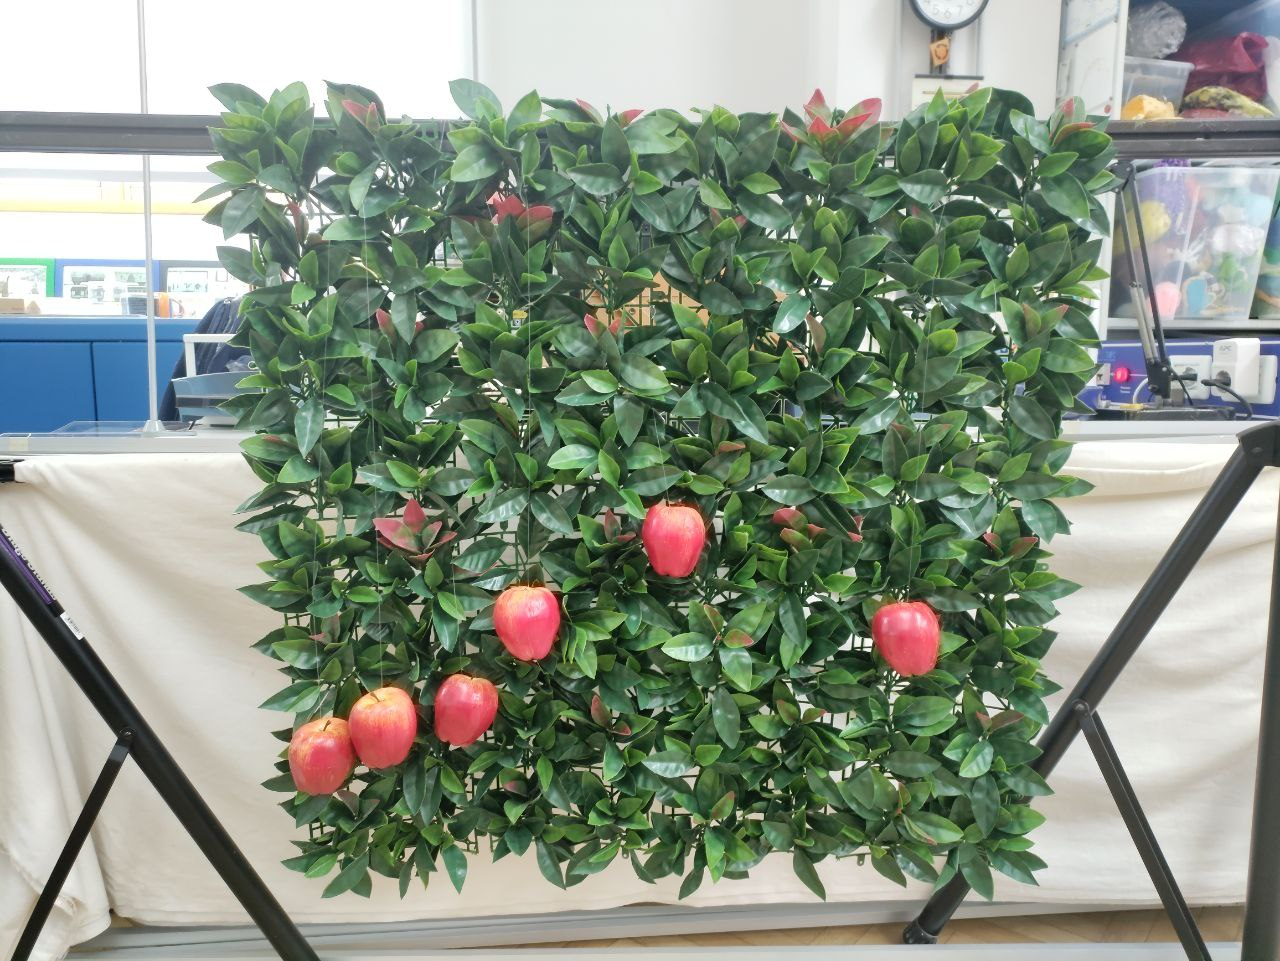
\includegraphics[width=1\textwidth]{c5_01.jpg}
        \caption{Simulated espalier apple tree}
        \label{fig:sim_espalier}
    \end{subfigure}
    \hfill % Optional: Adds space between images
    \begin{subfigure}{0.5\textwidth}
        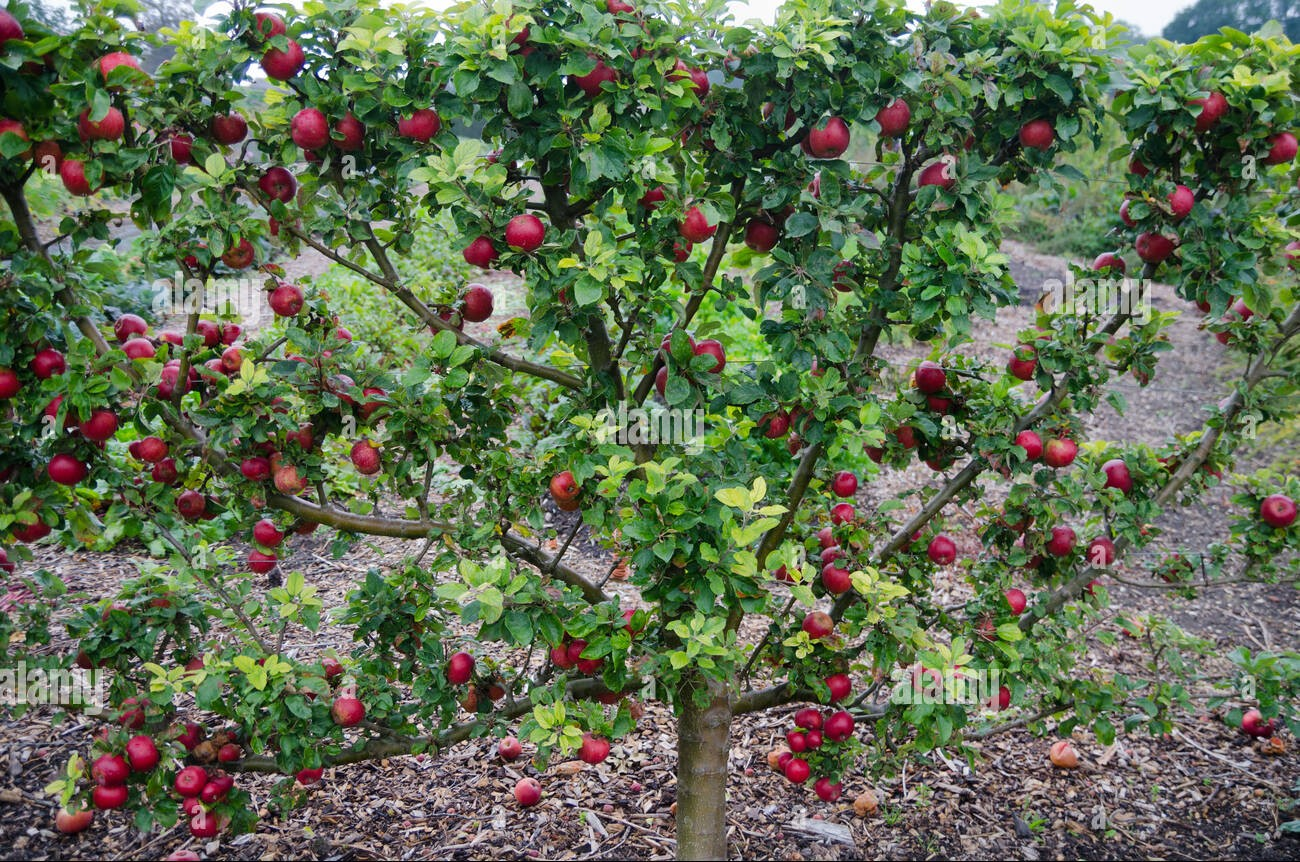
\includegraphics[width=1\textwidth]{c5_06.jpg}
        \caption{Real espalier apple tree}
        \label{fig:real_espalier}
    \end{subfigure}
    \caption{Espalier apple trees}
    \label{fig:plants}
\end{figure}

% Add a picture of colored balls on an artificial plant
\begin{figure}[t]
    \centering
    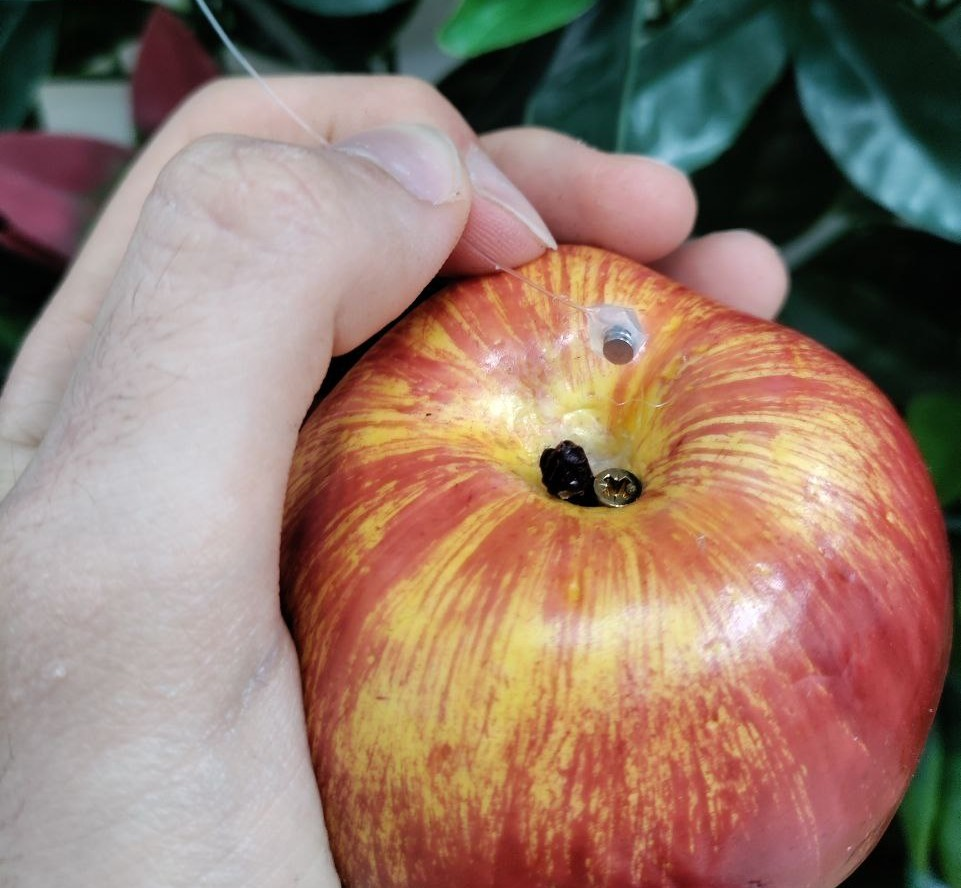
\includegraphics[width=0.5\textwidth]{c5_03.jpg}
    \caption{Magnetic attachment of an apple to the nylon string}
    \label{fig:magnetic}
\end{figure}

The colored balls and apples are attached to the plant with a nylon string. At the extremity of the string, 
a small magnet is secured using two different methods:

\begin{itemize}
    \item \textbf{Version 1 (Hot Glue)}: the magnet is attached to the string with hot glue. 
    For the apples, the magnet is attracted to another magnet placed on a screw that is screwed into the plastic apple. 
    In the case of the colored balls, the magnet is attracted to another magnet glued onto the ball. 
    To enhance robustness, the balls have two magnets: one inside and one glued onto the external surface. 
    Figure \ref{fig:magnetic} shows the magnetic attachment of an apple to the nylon string.
    \item \textbf{Version 2 (3D Printed Magnetic Hook)}: the second iteration replaces the hot glue with a 3D printed hook. 
    This version is designed exclusively for the apples since they can accommodate the screw where the magnet is attached.
    The magnet is securely placed within the hook, without the need for hot glue, and the nylon string is wrapped around it,
    as shown in Figure \ref{fig:hook3dprint}. 
    This eliminates the need for hot glue, which can be unreliable when bonding to magnets, resulting in a more robust attachment.
    The 3D-printed hook is small and lightweight, maintaining the overall design's unobtrusive nature, and 
    ensuring very fast printing times and quick installation. The 3D design is shown in Figure \ref{fig:hookdesign}.
    It is printed in white PLA (Polylactic Acid), making it strong and durable, with a smooth surface finish.
\end{itemize}

Both versions are effective in attaching the objects to the plant and making them detachable without excessive force,
allowing the robotic arm to easily detach them without straining the motors. 
The magnets are small and lightweight, minimally impacting the object's weight and shape. 
The nylon string is thin and transparent, remaining invisible to the camera and preserving the object's appearance.
The key advantage of the 3D printed hook (Version 2) is its enhanced reliability and ease of assembly compared to 
the hot glue method (Version 1).

% Add a picture of the magnetic attachment to apples and balls
\begin{figure}[t]
    \centering
    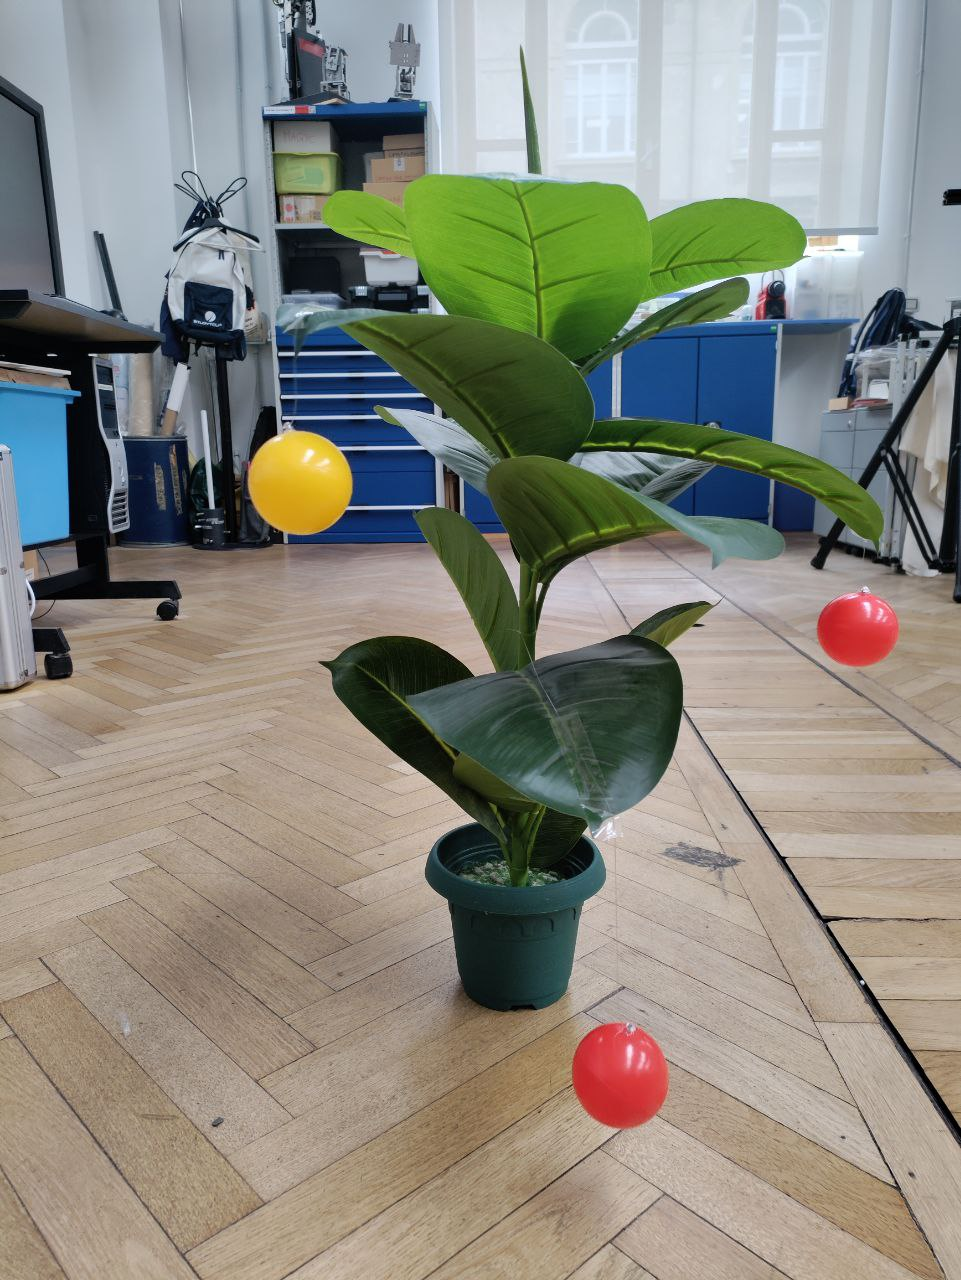
\includegraphics[width=0.6\textwidth]{c5_04.jpg}
    \caption{Simulated plant with colored balls}
    \label{fig:sim_plant}
\end{figure}

%add screenshot of apple hook 3d print and real apple with hook
\begin{figure}[ht]
    \centering
    \begin{subfigure}{0.55\textwidth}
        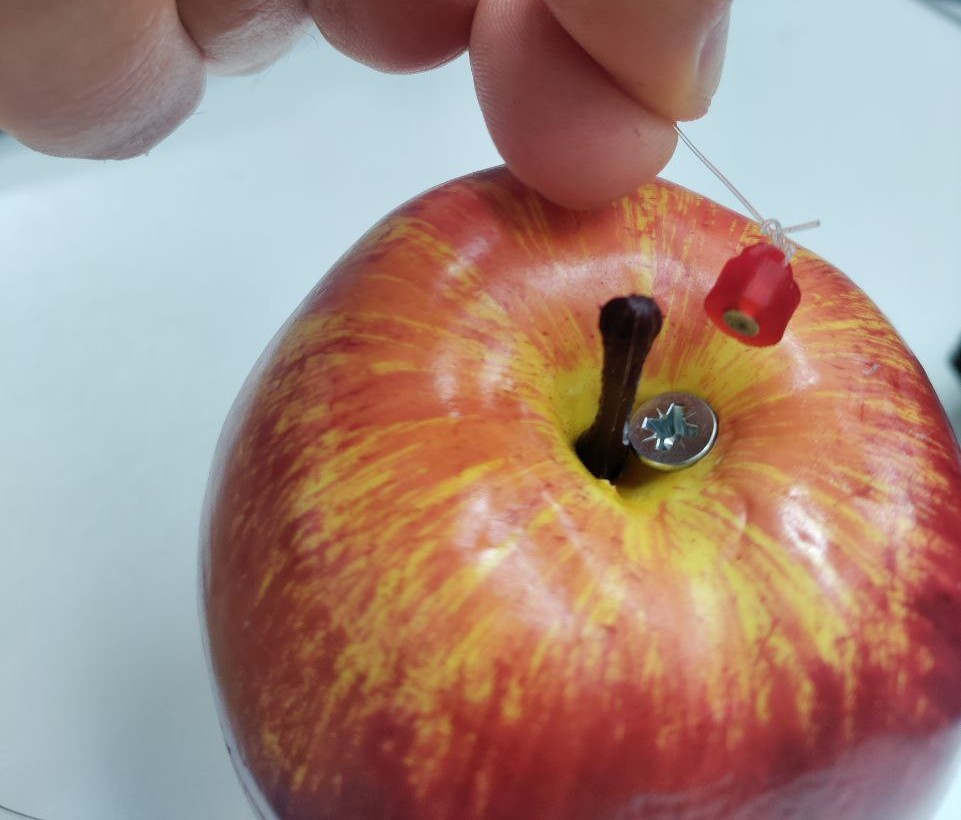
\includegraphics[width=1\textwidth]{c5_20.jpg}
        \caption{Magnetic 3D-printed hook on an apple}
        \label{fig:hook3dprint}
    \end{subfigure}
    \hfill % Optional: Adds space between images
    \begin{subfigure}{0.4\textwidth}
        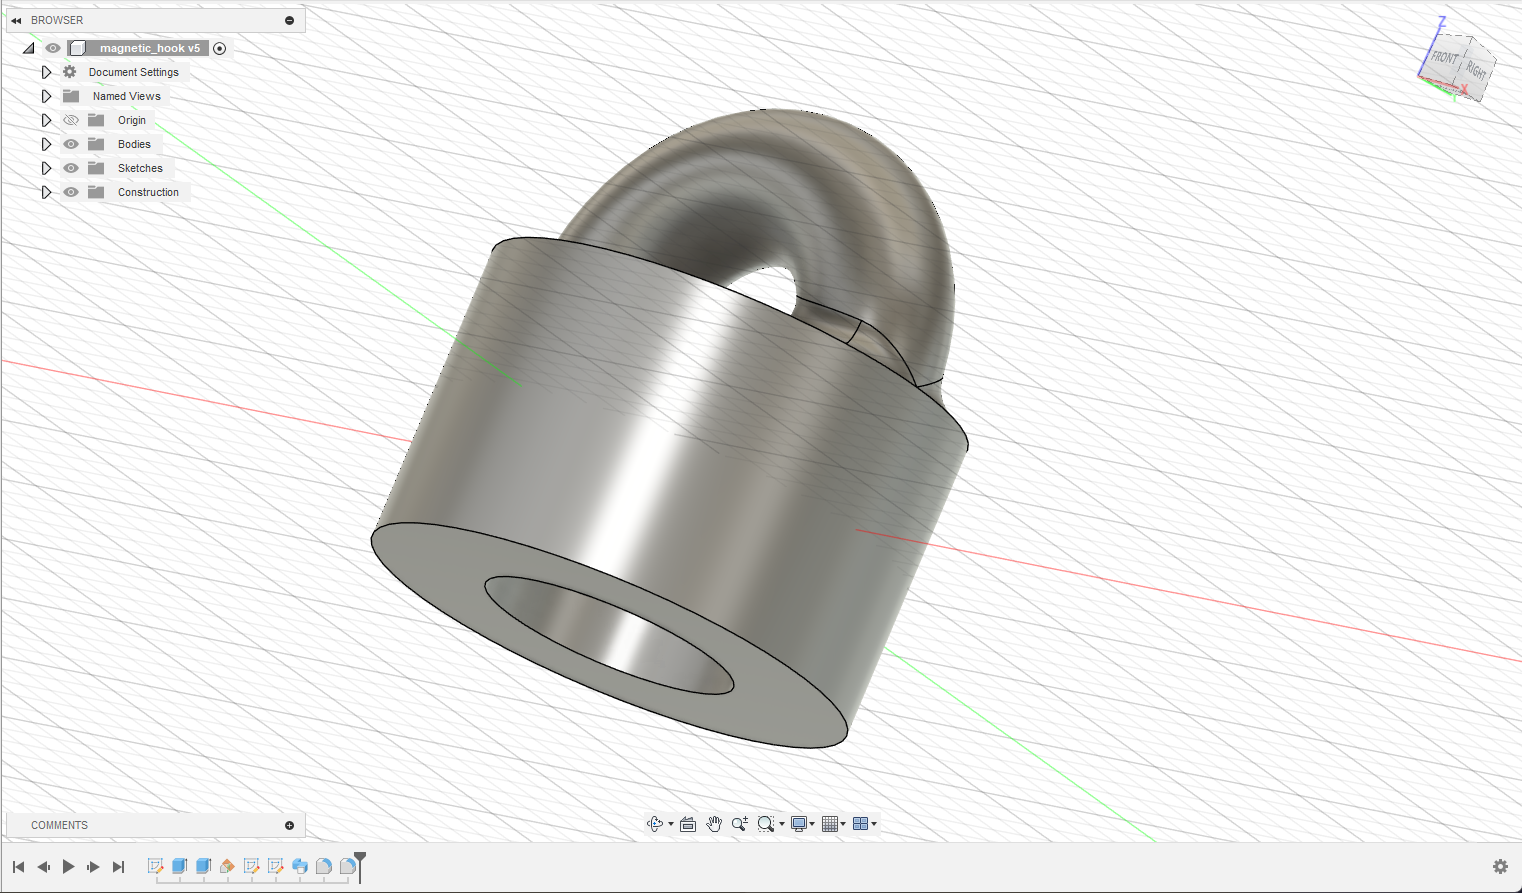
\includegraphics[width=1\textwidth]{c5_22.png}
        \caption{Magnetic hook 3D design}
        \label{fig:hookdesign}
    \end{subfigure}
    \caption{Magnetic hook for attaching apples}
    \label{fig:hook}
\end{figure}

\subsection{DemoV1 with Manual User Input}

This first version of the demo (\textit{DemoV1}) is a test for the grasping capabilities of the soft gripper and
the autonomous control of the robotic arm, without any advanced perception algorithm implemented. 
This demo is also meant to be used when the robotic arm is fixed in a specific location. The demo consists of
the robotic arm picking colored balls from the artificial plant, with manual user input for selecting the target
object to be picked. The user selects the target object by clicking on the object in the camera's field of view,
and the robotic arm moves to the target object's position and grasps it. The user can select only one object at 
a time.

When starting the demo, an image window appears on the screen, showing the camera's RGB image feed.
The user can \textbf{click on the image} and the coordinates of the mouse click are recorded, and broadcast on a ROS2
topic. The object that the user clicks on is assumed that it can be approximated as a sphere.
The algorithm for object position estimation computes the object's position in the camera frame
using the pixel coordinates, the camera's intrinsic parameters, and the depth image from the infrared camera.
The result is a $(x, y, z)$ position vector of the visible point clicked by the user in the camera frame. 
This is the point of the pointcloud on the surface of the object, which roughly corresponds to the 
object's visible surface center. By projecting a ray from the camera's optical sensor to the computed point,
the algorithm computes the object's approximate center in the camera frame. The center is then transformed
into the robot's base frame, and used as input to the grasping pose estimation algorithm to compute the target pose
for the end effector required to position the robot where the object can be grasped.

Once the grasping pose is computed, the robot moves to the target pose and the end effector grasps the object.
The robot then moves to a standard pre-defined position and drops the object, assuming that a basket
is placed exactly underneath the robot's end effector in the dropping position. The robot then returns to the
starting position and waits for the user to select the next object to be picked. Figure \ref{fig:bp1}
shows this demo during its execution, using colored balls as objects to be grasped. The demo worked well
both with the balls attached to the simulated tree and with the ball in the hands of human volunteers, as
in Figure \ref{fig:bp1}.

\begin{figure}[t]
    \centering
    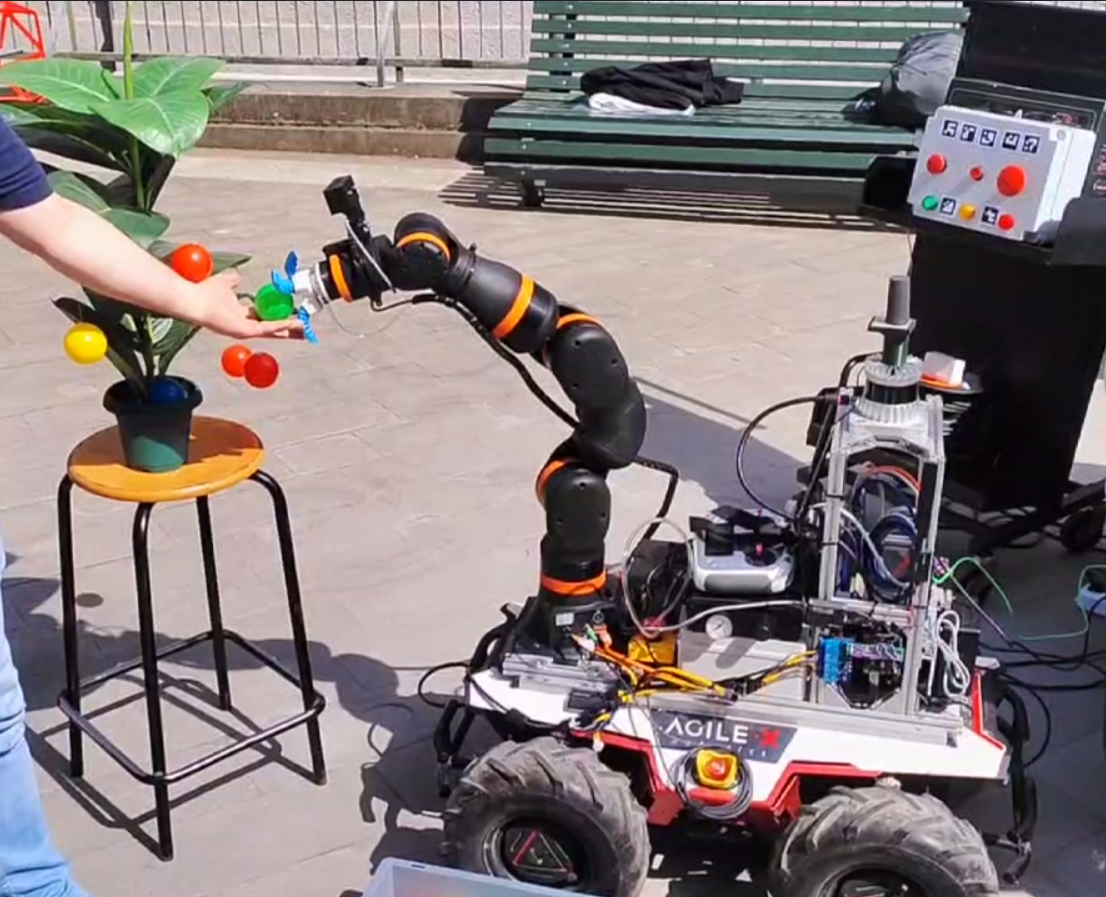
\includegraphics[width=1.0\textwidth]{c5_13.png}
    \caption{Cobot grasping a colored ball from the hand of a volunteer}
    \label{fig:bp1}
\end{figure}

One of the issues faced during the development of the \textit{DemoV1} for ball picking was the \textbf{reflectivity} of the balls
in the \textbf{infrared spectrum} in the presence of strong sunlight. The balls were reflecting the sunlight and the infrared
camera was not able to compute the depth in the spots of the balls' surface with the highest reflectivity. This resulted
in the balls' surface appearing as holes in the depth image. So if the user clicks exactly in the spot where
the ball is very reflective, the depth value computed would be either wrong or infinite and would result in the
algorithm crashing or computing an infeasible grasping pose. This effect was more pronounced with yellow balls.
The immediate solution is to click in the least reflective spots, but this is a temporary workaround and 
not a definitive solution to the problem. \textit{DemoV2} offers a more robust solution to this problem.

\subsection{DemoV2 with Object Detection Neural Network}

In demo version 2 (\textit{DemoV2}), the demo does not require any user input for selecting the object to be picked.
Instead, it relies on a neural network for detecting the objects in the camera's field of view. 
The neural network used for the object detection task is described in section \ref{sec:yolov8}.
The YOLOv8 neural network
is trained to detect the colored balls and the apples, and it outputs the object's bounding box and class label
with the confidence score. The predicted bounding box is used as the starting point to obtain a pointcloud
containing the points on the entire object's surface. The pointcloud is then used to compute the object's center
in the camera frame, and the grasping pose is computed as in the previous version of the demo.
The algorithm \ref{alg:sphere} assumes that the object can be approximated as an ideal sphere of known radius.
This algorithm is very robust for the colored balls, since they are spheres, and less robust and reliable
for the apples, because of their irregular shape. The algorithm is able to compute the object's center
even from a small portion of the object's surface, and this is a key feature of the algorithm because
it does not require the entire object to be visible in the camera's field of view.

DemoV2 solved the infrared reflectivity problem because it relies on the entire pointcloud of the object's surface, and not just
on a single point. This means that even if there is a hole in the pointcloud, the algorithm \ref{alg:sphere} is still able
to compute the object's center correctly (even though likely less precisely).
In the cases where the pointcloud presents points with wrong depth values, the algorithm
is still able to find the correct solution, as RANSAC is robust to outliers and noise in the data.

DemoV2 is programmed to take into account the \textbf{slow performance of the neural network} during inference
on the CPU. The neural network runs on the CPU and it is not able to process the images fast enough to provide
real-time object detection. The neural network takes around 0.5 seconds to process a single image
on the Intel NUC onboard computer, when other algorithms and ROS2 nodes are running in parallel,
especially during the execution of the complete demos. 
Since the task is not time-critical, the neural network can run in the background and provide the predictions
as soon as they are available. The code is implemented with multiple parallel threads that can handle 
and synchronize the data flow between the neural network and the other algorithms.
The code uses the predictions from the neural network coupled with the depth and RGB
images taken at the moment of inference.


\subsection{Mobile Fruit Picking Demos}

\begin{figure}[hpt]
    \centering
    \begin{subfigure}{\textwidth}
        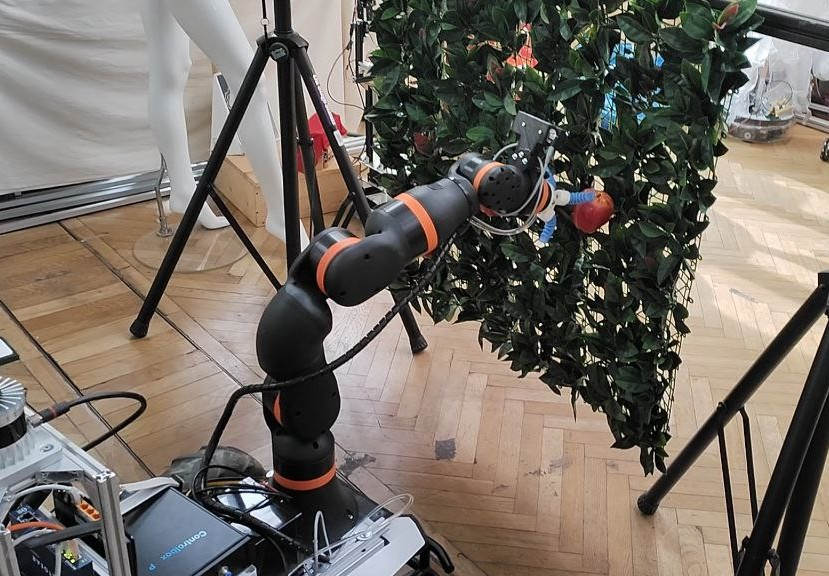
\includegraphics[width=1.0\textwidth]{c5_14.jpg} % Replace with your image file
        \caption{The cobot opens the gripper in the proximity of the apple (at the computed grasping pose) to grasp it}
        \label{fig:mfp1}
    \end{subfigure}
    
    \vspace{1em} % Add some vertical space between images (adjust as needed)

    \begin{subfigure}{\textwidth}
        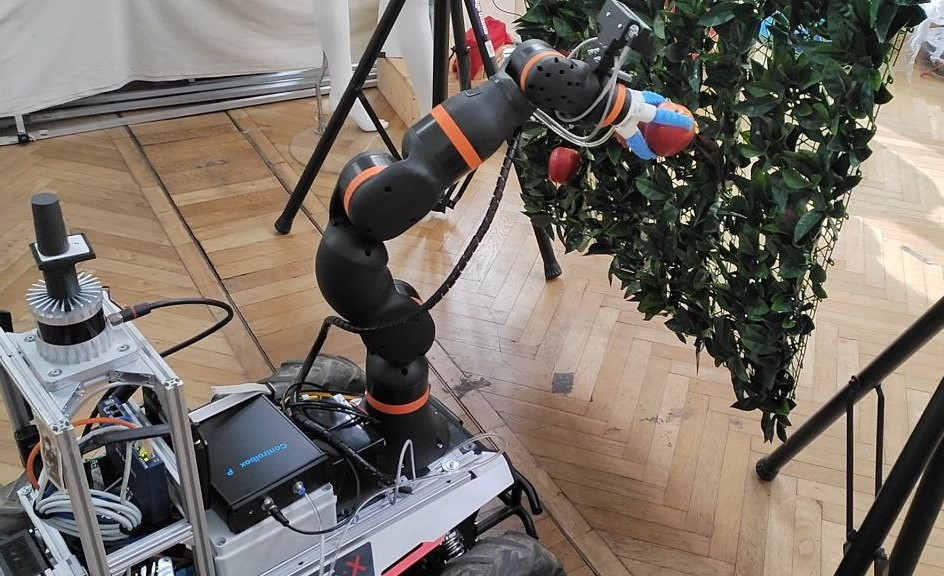
\includegraphics[width=1.0\textwidth]{c5_17.jpg} % Replace with your image file
        \caption{The cobot grasps the apple from the plant}
        \label{fig:mfp2}
    \end{subfigure}

    \caption{Mobile Fruit Picking demo during execution}
    \label{fig:mfp_}
\end{figure}

The \textbf{complete demo} is based on DemoV2 and extended to include the mobile base's navigation and obstacle avoidance
capabilities. The demo consists of the mobile manipulation robot navigating to the apple tree's location, detecting the apples
using the neural network, and picking the apples in a predefined sequence.
Figure \ref{fig:mfp_} shows different stages of the execution of this demo, where the robot is picking an apple from the tree.
The robot then drops the apples into a basket. There are two versions of the complete demo:

\begin{enumerate}
    \item \textbf{DemoV2 with pick and place on robot}: the robot picks the apples from the tree and drops them on
    a basket that is positioned on the mobile robot base.
    Figure \ref{fig:mobilebasket} shows the basket positioned on the mobile robot base, with the apples collected
    from the tree using the described sequence of actions. The robot does not need to navigate to a separate location
    to drop the apples, but it is sufficient for the robotic arm to move to a predefined position so that
    the end effector is immediately above the basket. This version is simpler and less challenging than the first one,
    but it was implemented to have a demo that is faster to execute and more realistic of a real-world scenario
    where the robot would operate in an agricultural field.
    \item \textbf{DemoV2 with pick and place}: the robot picks the apples from the tree and navigates to a predefined
    location to drop the apples in a basket. The basket is located in a position separate from the tree, and the robot
    must navigate to the basket's location to drop the apples. The robot must avoid obstacles in the environment
    while navigating to the basket's location. This version is more complex and challenging because the robot must
    navigate to two different locations. Once the mobile robot parks next to the basket's location, the robotic
    arm searches with the camera for an ArUco marker, which signals the position of the basket. 
    The basket with the ArUco signal marker is shown in Figure \ref{fig:basket}. Then
    an algorithm finds a feasible pose for the end effector such that it gets placed immediately above the basket,
    where it can release the grip on the grasped object and drop it, as shown in Figure \ref{fig:mfp3}.
    The sequence of actions executed for this demo is shown in the flowchart in Figure \ref{fig:mfp_flowchart}.
\end{enumerate}

\begin{figure}[t]
    \centering
    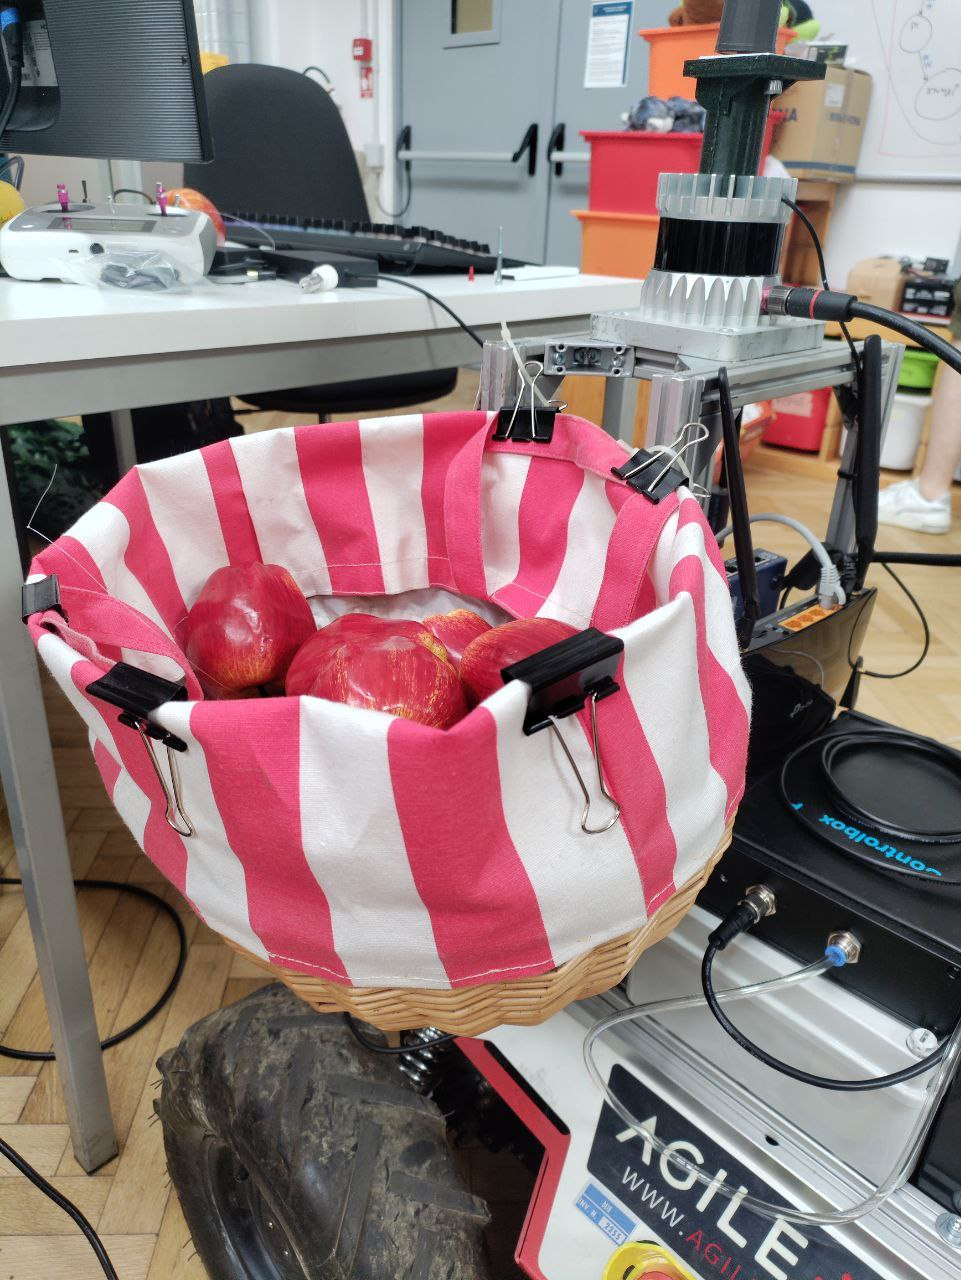
\includegraphics[width=0.5\textwidth]{c5_21.jpg}
    \caption{Basket positioned on the mobile robot base}
    \label{fig:mobilebasket}
\end{figure}

\begin{figure}[hpt]
    \centering
    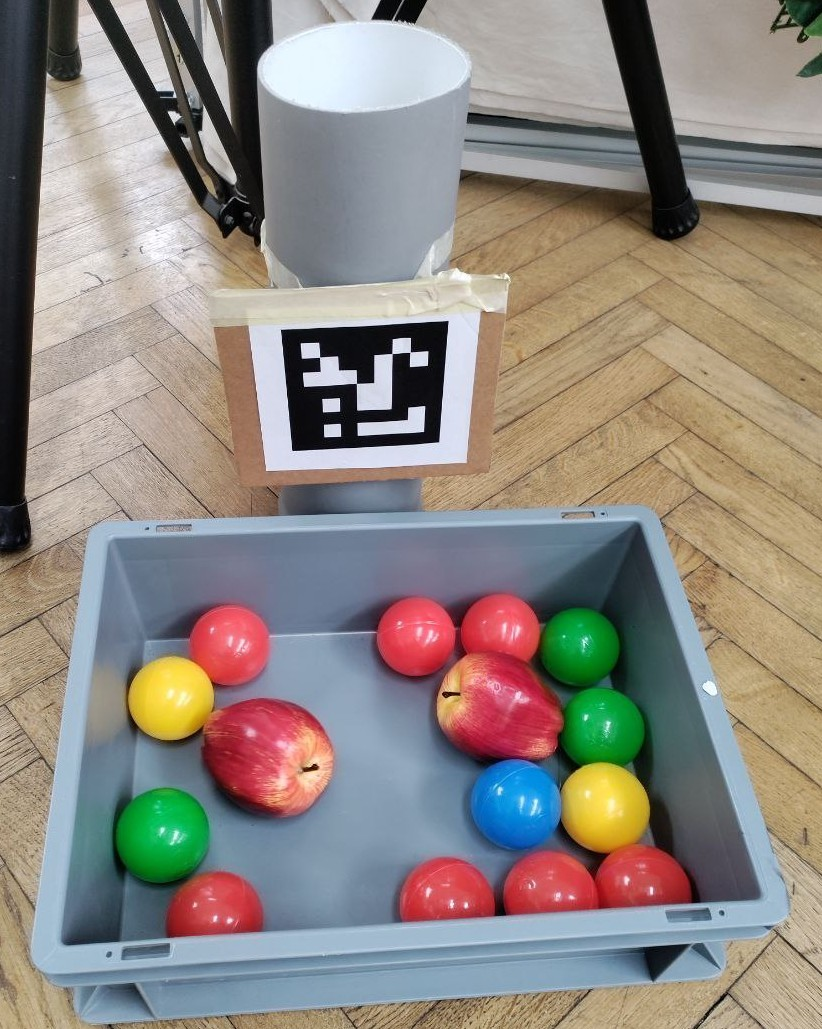
\includegraphics[width=0.5\textwidth]{c5_02.jpg}
    \caption{Basket at the dropping location}
    \label{fig:basket}
\end{figure}

\begin{figure}[hpt]
    \centering
    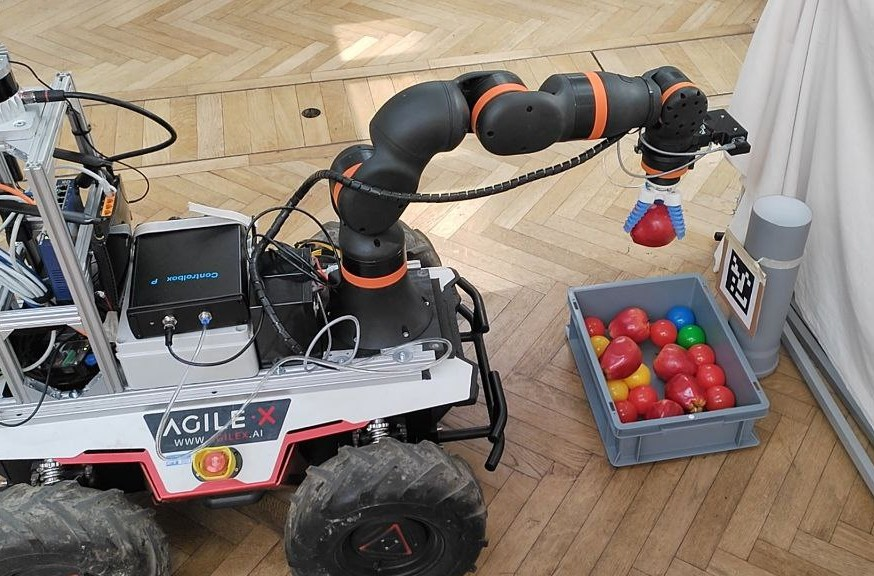
\includegraphics[width=1.0\textwidth]{c5_18.jpg}
    \caption{Cobot dropping the apple in the basket, at the dropping location, during the mobile fruit picking demo}
    \label{fig:mfp3}
\end{figure}

\begin{figure}[hpt]
    \centering
    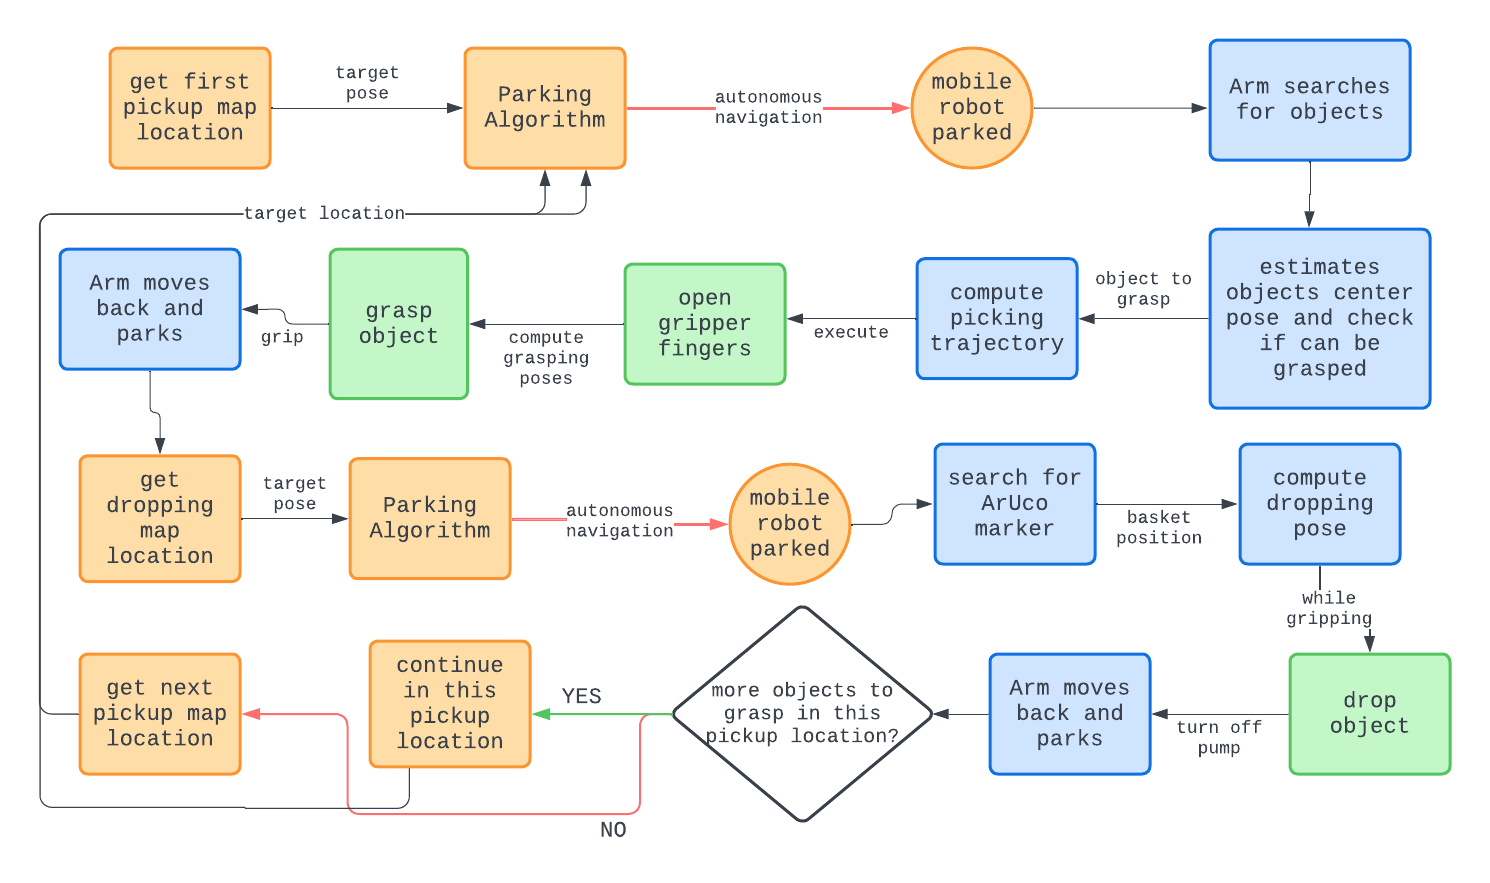
\includegraphics[width=1.0\textwidth]{demo2.png}
    \caption{Flowchart for the Mobile Fruit Picking Demov2 with pick and place}
    \label{fig:mfp_flowchart}
\end{figure}

The \textbf{object picking routine}, explained in algorithm \ref{alg:picking} is the routine that the robot follows
to pick up objects from a plant. This algorithm is suitable for both apples and colored balls since they are
both approximated as spheres. This routine defines the sequence of actions to be executed by the robot
to search for an object to pick, grasp, and drop in a basket, which can be located either on the robot itself
or in a separate location far from the tree.
The picking routine differs based on the version of the demo. When the robot must place the object
in the basket positioned on the mobile robot itself, or just next to the robot itself, the robotic arm moves to
the dropping pose and drops the object, as explained in the algorithm \ref{alg:picking}. Instead, when the robot
must pick and place in separate locations, the robotic arm moves to its parking position and does not release the object
until the mobile base has reached the dropping location and the camera recognizes the basket using the ArUco marker.

\begin{algorithm}[hp]
    \caption{\textbf{Object Picking Routine}}
    \label{alg:picking}
    \begin{algorithmic}[1]
        \Require Neural Network for object detection \textit{NN}
        \Require Depth Image feed $D$
        \State max object distance $z_{max} = 1.5$ in meters
        \State Generate a list of pose waypoints $W$
        \For {each waypoint $w$ in $W$}
            \State plan and execute trajectory from current pose to $w$
            \State check if there are objects detected by \textit{NN}
            \For {each object $o$ detected by \textit{NN}}
                \State compute \textbf{segmented pointcloud} using algorithm \ref{alg:sphere}
                \State compute centroid point $P$ from segmented pointcloud
                \State compute distance $z$ from centroid $P$
                \State get confidence score $c$ of object $o$ from vector $C$
                \State compute \textbf{priority score} $s = c \cdot 1/4 + (z_{max} - z)/z_{max} \cdot 3/4$
            \EndFor
            \State Choose object $o$ having highest score $s$
        \EndFor
        \State Estimate \textbf{object's center} using algorithm \ref{alg:sphere}
        \State Estimate \textbf{grasping pose} $G$ using algorithm \ref{alg:grasping}
        \If {$\exists$ feasible pose $G$}
            \State compute pre-grasping pose $G'$
            \State plan and execute trajectory to $G'$
            \State \textbf{open the gripper}
            \State plan and execute linear trajectory from $G'$ to $G$
            \State \textbf{close the gripper} to grasp the object
            \State plan and execute linear trajectory from $G$ to $G'$
            \State move back to waypoint $w$
            \State move to dropping pose $d$
            \State \textbf{open the gripper} to drop the object
            \State \textbf{turn off the gripper}
        \Else
            \State move to next waypoint
        \EndIf
    \end{algorithmic}
\end{algorithm}

The algorithm \ref{alg:picking} is the main algorithm that the robot follows to pick objects from the tree.
The algorithm is executed for each waypoint in the list of poses that the robot must follow to search
for objects to pick. If there are multiple objects detected by the neural network in a unique searching pose,
the algorithm chooses the object with the highest priority score, which is computed based on the object's distance
from the robot and the confidence score of the object's detection. The priority score is used to choose the object
that is closest to the robot and has the highest confidence score. The algorithm then computes the object's center
and the grasping pose, and it executes the trajectory to grasp the object. The robot then moves to the dropping pose
and drops the object into the basket. 

\subsection{Mobile Fruit Picking Demo Implementation and Architecture}
\label{sec:demo2}

This complete demo requires the \textbf{integration of multiple software components},
such as the neural network for object detection,
the perception algorithms for computing the object's center, the grasping pose estimation algorithm, the trajectory
planning algorithms, and the navigation and obstacle avoidance algorithms. The demo is a complex orchestration of
multiple algorithms wrapped in ROS2 action servers. The action servers are responsible for executing the actions
and the algorithms required to pick the objects. The action client node is responsible for orchestrating the actions
of the mobile base and the robotic arm, and for sending the goals to the action servers. The action client node
also handles the sequence of actions in case of any failure of any software component and logs the feedback data
received from the action servers. The ROS2 action servers used in the demo are:

\begin{itemize}
    \item \textbf{Parking Action Server}: this server is the same as the one used for the other complete demo.
    The only difference with the other demo is that the location from which the robot must compute
    the parking position is not given by the result of another action, but is read from a configuration file.
    Both poses where to pick objects and the dropping location are hardcoded in a configuration file for
    simplicity and ease of use.
    \item \textbf{Picking Action Server}: this server is responsible for executing the first part of the
    object-picking routine. It is responsible for searching for objects to pick and checking whether there
    exists a feasible grasping pose for the objects in the camera frame. If it finds a feasible grasping pose
    for an object, it plans and executes the trajectories to grasp the object. The server returns the result
    of the planning and execution of the trajectories. It also provides logging feedback about the objects
    detected and the grasping poses computed.
    \item \textbf{Dropping Action Server}: this server is responsible for executing the second part of the
    object-picking routine. It is responsible for moving the robot to the dropping location and dropping the object
    into the basket. This server is called only if the dropping location is separate from the picking location.
    It searches for an ArUco marker signaling the dropping location and computes a feasible pose for the end effector
    to drop the object. Then it moves to that pose and drops the object.
    The server returns the result of the execution of the trajectories and the dropping action.
    It also provides logging feedback about finding the ArUco signaling the dropping location. 
\end{itemize}

The architecture of the whole system is composed of multiple software components that interact with each other
using ROS2 Actions, Services, and Topics. The architecture, shown in Figure \ref{fig:arch2}, is designed to be modular
and scalable, to allow the integration of new components and functionalities in the future.
The architecture is composed of the following macro components:

\begin{itemize}
    \item \textbf{ROS2-Control Gripper Interface}: this component is responsible for actuating the soft gripper,
    using a ROS2 service as an interface to the gripper's ROS2 hardware interface. The hardware interface
    used has a structure analogous to the one used for the control of the robotic arm, as described in 
    section \ref{sec:ros2control}. The ROS2 service is handled by the MoveIt2 APIs node, which provides
    a convenient interface to couple the trajectory planning and execution with the gripper's control,
    necessary for the manipulation tasks.
    \item \textbf{MoveIt2 Servers}: this component includes the MoveIt2 Planning and Execution functionalities
    and the two action servers for finding the parking pose and pressing the buttons. The MoveIt2 servers
    are responsible also for computing and executing the linear trajectories generated by the trajectory planner,
    required for grasping the detected objects. These servers handle also the perception algorithms for computing
    the object's center and the grasping pose, as described in the section \ref{sec:perception}.
    They use the YOLOv8 neural network predictions to execute the pipeline of actions required to pick the objects. 
    The demo execution pipeline is handled within threads executed
    on-demand by the MoveIt2 servers, given the goal sent by the client node.
    \item \textbf{Nav2 Servers}: this component is responsible for the autonomous navigation of the mobile base
    using Nav2. It includes also the action server for computing the parking algorithm and the action client
    exploiting Nav2 Commander APIs to send navigation goals to the mobile base. The structure of the parking algorithm
    is explained in section \ref{sec:parking}, while the autonomous navigation integration with ROS2 is explained
    in section \ref{sec:nav2}.
    \item \textbf{Client Node}: this component is responsible for orchestrating the actions of the mobile base
    and the robotic arm. The client node is a ROS2 node that integrates the action clients for the parking, button finder,
    and button presser action servers. The orchestration of the actions is handled by different threads that
    are executed on-demand by the client node, given the goal sent by the user. Multiple threads are present
    since each one is responsible for handling different tests and demo versions.
    \item \textbf{Neural Network Node}: this component is responsible for running the YOLOv8 neural network
    inference on the RGB images taken by the camera. The neural network node is a ROS2 node that subscribes
    to the RGB image topic and publishes the predictions on a ROS2 topic, as described in section \ref{sec:yolov8}.
    The neural network node is implemented as a wrapper around the Tensorflow model and uses the 
    Tensorflow Python API to load the model and run the inference.
    \item \textbf{ArUco Pose Estimation node}: this component is responsible for computing the ArUco markers' poses
    in the camera frame.
\end{itemize}

% Add a Picture of the diagram
\begin{figure}[ht]
    \centering
    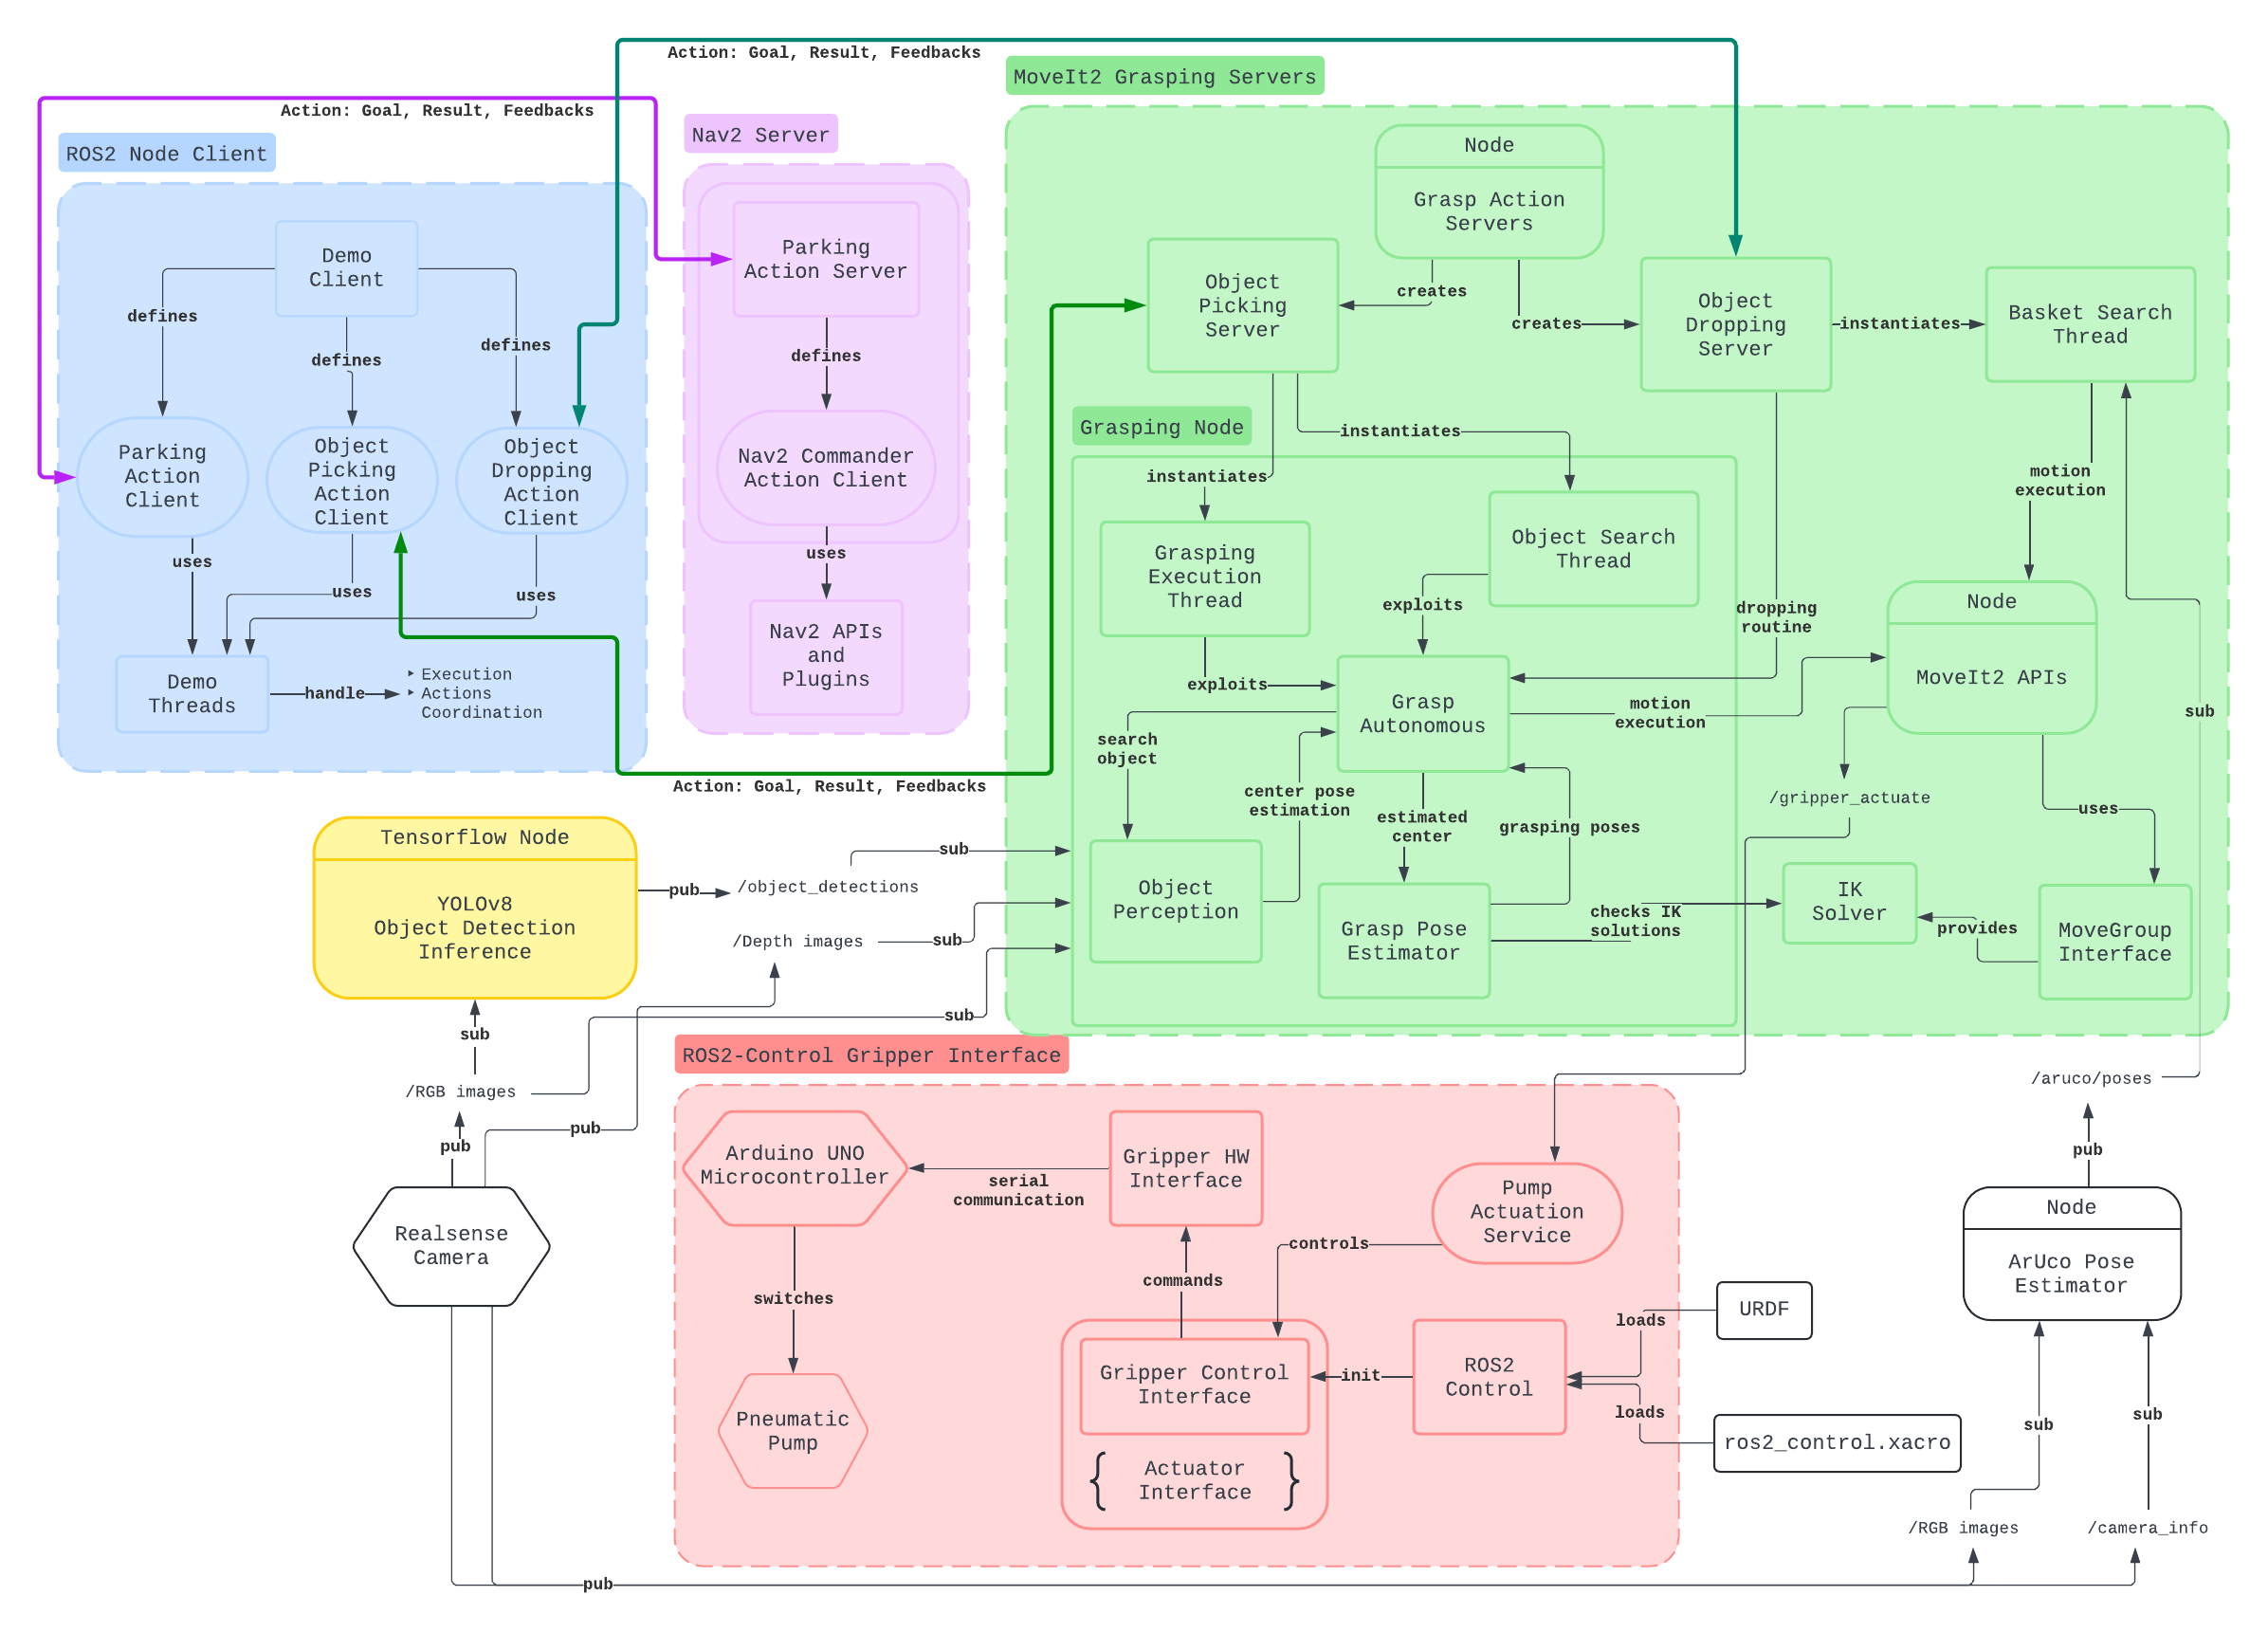
\includegraphics[width=1.0\textwidth]{Mobile Fruit Picking Demo_updated.png}
    \caption{Architecture diagram of the Mobile Fruit Picking demo}
    \label{fig:arch2}
\end{figure}


\addtocontents{toc}{\vspace{2em}} % Add a gap in the Contents, for aesthetic



\end{document}